\documentclass[aps,pre,twocolumn,superscriptaddress,floatfix]{revtex4-2}

\usepackage[utf8]{inputenc}
\usepackage[T1]{fontenc}
\usepackage{graphicx}
\graphicspath{{../../figures/}}
\usepackage{amsmath,amsthm}
\usepackage{amssymb}
\usepackage{nicefrac}
\usepackage{tikz}
\usepackage[section]{placeins}
\usepackage{hyperref} % hyperref should be loaded late
\usepackage{cleveref}
\usepackage{subcaption}
\usepackage{orcidlink}
\usepackage{booktabs}

%\usetikzlibrary{positioning,arrows.meta,fit,calc}

\begin{document}

% --- Document Information ---
\title{
Simulation-Based Inference for Plant-Wide Fault Diagnosis and 
Artefactual Non-Identifiability Under
Closed-Loop Control
}

\author{Simone Casolo \orcidlink{0000-0003-2945-8931}
}
\email{simone.casolo@cognite.com} 
\affiliation{Cognite AS, Oslo, Norway}

\author{Alexander Johannes Stasik \orcidlink{0000-0003-1646-2472}}
%\email{alexander.stasik@sintef.no} 

\affiliation{Department of Data Science, Norwegian University of Life Sciences, \AA s, Norway}
\affiliation{Department for Mathematics and Cybernetics, SINTEF Digital, Oslo, Norway}


\author{Signe Riemer-Sørensen\orcidlink{0000-0002-5308-7651}
}
\affiliation{Department for Mathematics and Cybernetics, SINTEF Digital, Oslo, Norway}

\date{\today}


\begin{abstract}
Fault diagnosis in feedback-controlled chemical processes is fundamentally
limited by the controller's tendency to compensate for degradation,
suppressing the parametric signatures that estimation methods rely on. We apply simulation-based inference
(SBI) across two systems of increasing complexity: a
PI-controlled CSTR (two fault parameters) and the Luyben
reactor-column-recycle benchmark (five fault parameters, three PI loops,
liquid recycle). SBI approximates the Bayesian posterior over degradation parameters by a neural spline
 flow trained on summary statistics of fixed-length
observation windows.
Identifiability is characterised via Fisher information
analysis, validated with simulation-based calibration, and benchmarked
against extended Kalman filter and Markov chain Monte Carlo baselines.
For the CSTR, the matched closed-loop posterior accurately recovers catalyst decay
and jacket fouling in non-saturating scenarios, while local sensitivity analysis
shows that PI temperature control makes jacket conductance less well conditioned than
catalyst activity. Severe fouling introduces actuator-saturation undercoverage, and
temperature-measurement bias creates a practical mild-fouling confound near the
classification boundary.
For the recycle plant, three apparent joint non-identifiabilities under summary-
statistic compression are shown, using a raw-trajectory Fisher-information check, to 
be representation artefacts rather than plant-level limitations. In contrast, 
thermal masking by integral temperature control remains a genuine representation-
independent information loss.
We show that confounds of comparable magnitude can have very different
operational consequences, depending on the fault taxonomy.
Furthermore, we show that amortised SBI can perform closed-loop, multi-unit fault 
identification directly from simulator-generated training data, without historical 
labelled-fault records.
SBI relies only on a simulator and is applicable when no tractable likelihood exists. 
It can represent joint, non-Gaussian posterior structure induced by closed-loop
recycle dynamics, while amortising inference to real-time monitoring cadence.
\end{abstract}

\maketitle

\noindent\textbf{Keywords:} condition monitoring, Bayesian statistics, 
simulation-based inference, predictive maintenance, closed-loop identifiability, recycle process, 
prognostics and health management, fault diagnosis.

\section{Introduction}
\label{sec:related_work}
\begin{figure*}[t]
    \centering
    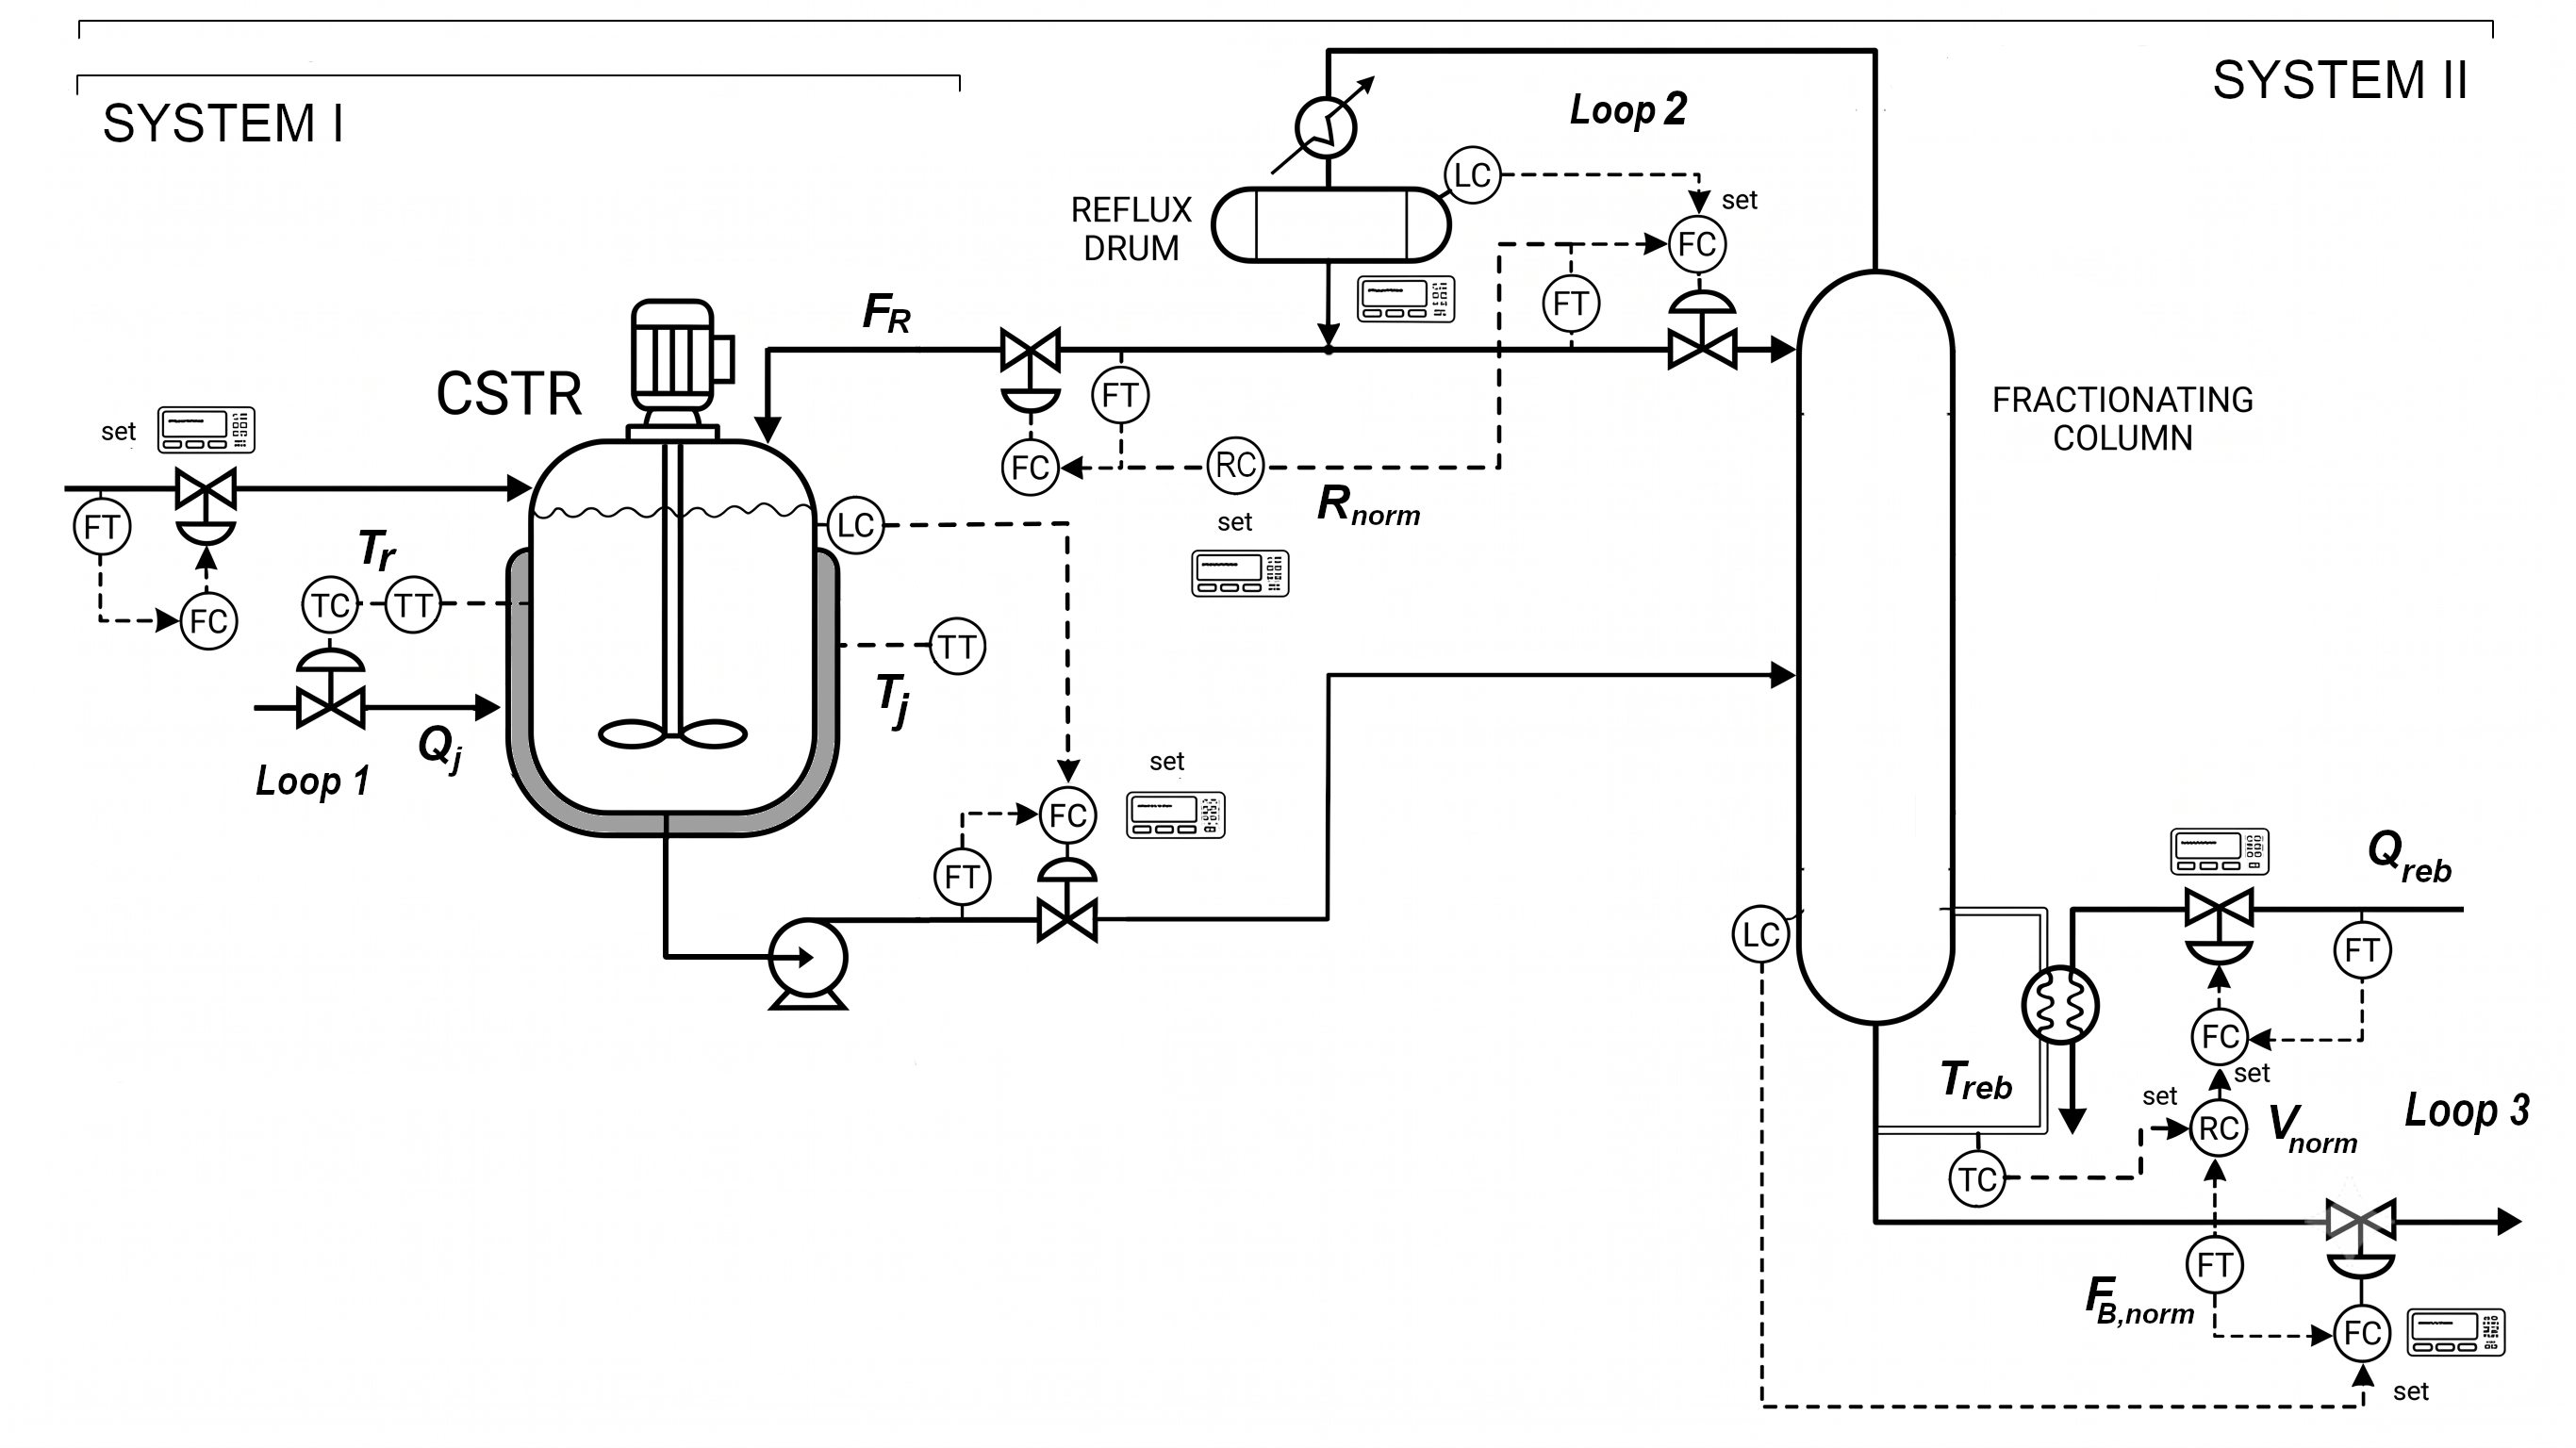
\includegraphics[width=0.9\linewidth]{PFD_Wu2003.png}
    \caption{Schematic of the two process systems studied.  System~I (left) 
     is a single propylene oxide CSTR under PI temperature
      control.  System~II (full diagram) is the Luyben reactor-column-recycle
      benchmark~\citep{Wu2003} consisting of a CSTR coupled to a distillation column
      with liquid recycle and three decentralized PI loops.}
    \label{fig:system_schematic}
\end{figure*}

Continuous chemical processes such as reactor-separator-recycle configurations
are subject to progressive degradation: catalyst activity decays through
poisoning or sintering, heat-exchanger surfaces accumulate fouling deposits,
and separator efficiency erodes over operating cycles. Digital twins 
can provide a real-time, physics-informed digital representation of these processes, 
enabling predictive maintenance and proactive fault 
management~\citep{REBELLO2025109178,DAOUTIDIS2024108523}.\\
Timely quantification
of such degradation is essential for risk-informed maintenance scheduling,
product quality assurance, and avoidance of unplanned shutdowns~\citep{Frank1990,Isermann2006}.
Current industrial practice relies on a few broad families of tools for the diagnosis of process faults~\citep{ZHAO2026112159, Huo2026}:
soft sensors, which regress fault parameters from process measurements but
do not provide uncertainty quantification~\citep{KADLEC2009795, PERERA2023105988},
model-based observers, principally the extended and unscented Kalman filters
(EKF/UKF), which propagate Gaussian approximations of the joint state-and-parameter
posterior~\citep{Jazwinski1970,JulierUhlmann2004},
multivariate statistical methods based on principal component analysis or
partial least squares, which provide sensitivity indices and alarms but not
calibrated parameter posteriors~\citep{Qin2012, Kini2024, Lou2021, Huo2026}, and
data-driven anomaly detectors built on neural or recurrent architectures,
which flag deviations from normal operation without quantifying fault severity in
physically interpretable units~\citep{WU2018185, Jia2025, Feng2026, HAN2020161, HAN20258859}.
None of these approaches delivers a calibrated
probability distribution over the fault-parameter space needed for maintenance planning. 
The decision to schedule an
intervention depends on the probability that a parameter has crossed a critical
threshold, not on whether a point estimate has done so.

This diagnostic task is made structurally harder by the feedback controllers
that regulate the plant. Decentralised proportional-integral (PI) loops
compensate for degradation.
%: a fouled heat exchanger is countered by increasing
%the coolant flow; a deactivating catalyst is compensated by adjusting the
%temperature setpoint.  
It is a well-understood limitation that the control compensation suppresses the same parametric
signatures that estimation methods rely on \citep{Gustavsson1977, Forssell1999}. 
Critically, this method-independent limitation is rooted in the information content
of the closed-loop data, and it affects Bayesian and frequentist, online and offline,
neural and classical methods equally (see~\citealt{Ljung1999}, Ch.~13). A fixed 
operating setpoint with a high-gain
controller implies near-zero spectral excitation of the controlled variable in the
frequency band where fault-parameter information is concentrated, driving the local
Fisher information for thermally-masked parameters toward zero. The practical
consequence for fault diagnosis is twofold: some parameters are fundamentally
harder to estimate than others under closed-loop operation, and apparent
joint non-identifiabilities that emerge in compressed feature representations may
be artefacts of lossy temporal aggregation rather than properties of the plant~\citep{s26123948}.  
Characterising and distinguishing these two effects (scalar information reduction versus
representation artefact) is the central methodological problem this work addresses.
Simulation-based inference (SBI)~\citep{Cranmer2020} is an attractive inference method in
this setting because it can approximate full Bayesian posteriors from simulator-generated
data without requiring a tractable likelihood. Its amortised form is especially relevant
for condition monitoring, where many observation windows must be processed repeatedly
after a single offline training stage. \\
This paper makes four contributions:
\emph{1}. It shows that faults in a PI-controlled CSTR can be recovered accurately in 
non-saturating regimes, while jacket fouling remains harder to quantify under saturation and temperature-measurement bias.
\emph{2}. It demonstrates amortised SBI for plant-wide fault identification in a 
closed-loop reactor-column-recycle benchmark with five degradation parameters, recycle 
coupling, and three decentralised PI loops.
\emph{3}. It introduces a raw-trajectory Fisher information diagnostic for distinguishing
representation artefacts from plant-level non-identifiability.
\emph{4}. It shows that the operational severity of a parameter confound depends on the 
downstream fault taxonomy, not only on the Fisher-information coupling magnitude.

\section {System~I: CSTR with PI Temperature Control}
\label{sec:system1}

Two systems of increasing complexity are studied. As shown in Figure \ref{fig:system_schematic}, System~I can be considered a sub-system of System~II, where System~I is a
single CSTR under proportional-integral temperature control, drawn from the canonical nonlinear CSTR benchmark of
Fogler~\citep{Fogler2016}. 
% with parameters representing propylene oxide hydrolysis reaction. 
%System~II is the Luyben
%reactor-column-recycle benchmark of~\citet{Wu2003} and depicted in 
%Fig.~\ref{fig:system_schematic}: a CSTR coupled to a distillation 
%column with liquid recycle and three decentralized PI loops.
%This section develops the full mathematical
%formulation for the two systems, motivates both the open- and closed-loop
%representations, and defines the fault parameterisation used throughout
%the study.
Specifically, we consider acid-catalysed liquid-phase hydrolysis of
propylene oxide (PO) to propylene glycol.
The reaction is pseudo-first-order in PO concentration, irreversible,
and mildly exothermic following an Arrhenius rate law.
Kinetic parameters are taken from Fogler
(2016), Module~13~\citep{Fogler2016}, whose values are traceable to the
original experimental measurements of \citet{Furusawa1969} for the
ring-opening of propylene oxide in dilute aqueous acid solution. 
%
%with pre-exponential factor $k_0 = 1.696\times10^{13}$~min$^{-1}$,
%activation energy $E_a = 75{,}362$~J~mol$^{-1}$, and universal gas
%constant $R = 8.314$~J~(mol~K)$^{-1}$.  

\subsection{Open-Loop Model}
\label{sec:open_loop}

In the absence of feedback control, the reactor is characterised by
three state variables: reactant concentration $C$~[mol~L$^{-1}$],
reactor temperature $T$~[K], and jacket temperature $T_c$~[K].  With
coolant flow rate $Q_c$ treated as a fixed external input, the
energy-balanced material model is
%
\begin{subequations}
\label{eq:open_loop}
\begin{align}
  \frac{dC}{dt}
    &= \frac{Q}{V}\bigl(C_i - C\bigr)
       - k(T)\,C,
  \label{eq:dC_ol} \\[4pt]
  \frac{dT}{dt}
    &= \frac{Q}{V}\bigl(T_i - T\bigr)
       - \frac{\Delta H_r}{\rho C_p}\,k(T)\,C
       - \frac{U\!A}{\rho C_p V}\bigl(T - T_c\bigr),
  \label{eq:dT_ol} \\[4pt]
  \frac{dT_c}{dt}
    &= \frac{Q_c}{V_c}\bigl(T_{ci} - T_c\bigr)
       + \frac{U\!A}{\rho_c C_{pc} V_c}\bigl(T - T_c\bigr).
  \label{eq:dTc_ol}
\end{align}
\end{subequations}
%

The reaction is exothermic, with $\Delta H_r = -84{,}666$~J~mol$^{-1}$. Under the sign convention of Eq. (1b), the heat-release contribution is therefore positive~\citep{Fogler2016,Ziyai2022,NIST_WebBook}. 
%As $\Delta H_r < 0$, the term $-\Delta H_r / (\rho C_p)$ in Eq.~\eqref{eq:dT_ol} is positive, reflecting the exothermic heat release. 
The overall heat transfer coefficient-area product $U\!A$ [cal~min$^{-1}$~K$^{-1}$] couples the reactor and jacket energy balances. All nominal parameter values are listed in Table~\ref{tab:params_system1}.

The open-loop steady state is found by setting all time derivatives to zero and solving the resulting nonlinear algebraic system.  At the
nominal operating conditions (Table~\ref{tab:params_system1}) and $Q_c = Q_{c0} = 80$~L~min$^{-1}$, the system has a unique physically
meaningful steady state at
$C_\mathrm{ss} \approx 0.018$~mol~L$^{-1}$,
$T_\mathrm{ss} \approx 312.5$~K,
$T_{c,\mathrm{ss}} \approx 299.1$~K,
corresponding to a single-pass conversion of approximately 98\%. The open-loop model captures the essential coupling between reactor exothermicity and jacket cooling, and serves as the reference for understanding how feedback control modifies the observable system behaviour.




% ------------------------------------------------------------------
\begin{table*}[tb]
\centering
\caption{Nominal parameter values for System~I (propylene oxide
  CSTR). Kinetic parameters from \citet{Fogler2016}
  (Module~13) based on \citet{Furusawa1969}, physical properties from
  \citet{PerrysHandbook}, controller tuning from the present work.}
\label{tab:params_system1}
\small
\begin{tabular}{lllll}
\toprule
Parameter & Symbol & Value & Units & Source \\
\hline
\midrule
\multicolumn{5}{l}{\textit{Reaction kinetics}} \\
Pre-exponential factor     & $k_0$          & $1.696\times10^{13}$ & min$^{-1}$            & \citet{Fogler2016} \\
Activation energy          & $E_a$          & 75{,}362             & J~mol$^{-1}$          & \citet{Fogler2016} \\
Standard heat of reaction  & $\Delta H_r$   & $-84{,}666$          & J~mol$^{-1}$          & \citet{Fogler2016,Ziyai2022} \\
Universal gas constant     & $R$            & 8.314                & J~(mol~K)$^{-1}$      & — \\
\midrule
\multicolumn{5}{l}{\textit{Reactor geometry and feed conditions}} \\
Reactor volume             & $V$            & 500                  & L                     & This work \\
Jacket volume              & $V_c$          & 40                   & L                     & This work \\
Volumetric feed flow       & $Q$            & 40                   & L~min$^{-1}$          & This work \\
Residence time             & $\tau = V/Q$   & 12.5                 & min                   & Derived \\
Inlet PO concentration     & $C_i$          & 0.97                 & mol~L$^{-1}$          & This work \\
Feed temperature           & $T_i$          & 297                  & K                     & This work \\
Coolant inlet temperature  & $T_{ci}$       & 297                  & K                     & This work \\
\midrule
\multicolumn{5}{l}{\textit{Physical properties}} \\
Reactor fluid density      & $\rho$         & 1{,}000              & g~L$^{-1}$            & \citet{PerrysHandbook} \\
Reactor fluid heat capacity & $C_p$         & 1.0                  & cal~(g~K)$^{-1}$      & \citet{PerrysHandbook} \\
Coolant density            & $\rho_c$       & 1{,}000              & g~L$^{-1}$            & \citet{PerrysHandbook} \\
Coolant heat capacity      & $C_{pc}$       & 1.0                  & cal~(g~K)$^{-1}$      & \citet{PerrysHandbook} \\
Heat transfer coefficient-area & $U\!A$     & 12{,}500             & cal~(min~K)$^{-1}$    & This work \\
\midrule
\multicolumn{5}{l}{\textit{PI controller}} \\
Temperature setpoint       & $T_\mathrm{sp}$ & 312.5               & K                     & This work \\
Proportional gain          & $K_p$          & 150                  & (L~min$^{-1}$)~K$^{-1}$ & This work \\
Integral time constant     & $\tau_i$       & 10                   & min                   & This work \\
Coolant flow bias          & $Q_{c0}$       & 80                   & L~min$^{-1}$          & This work \\
Coolant flow minimum       & $Q_{c,\min}$   & 0                    & L~min$^{-1}$          & Physical \\
Coolant flow maximum       & $Q_{c,\max}$   & 400                  & L~min$^{-1}$          & Physical \\
\midrule
\multicolumn{5}{l}{\textit{Fault parameter priors}} \\
Catalyst activity          & $\alpha$       & $\mathcal{U}(0.4,\,1.2)$ & — & This work \\
Jacket conductance         & $\beta$        & $\mathcal{U}(0.4,\,1.2)$ & — & This work \\
\hline
\bottomrule
\end{tabular}
\end{table*}
% ------------------------------------------------------------------

\subsection{Closed-Loop Model}
\label{sec:closed_loop}
%In industrial practice, continuous stirred-tank reactors operating at
%exothermic conditions are invariably equipped with feedback temperature
%controllers to prevent runaway and to maintain product quality.  
The closed-loop model employed in this work augments the open-loop
system in Eq.\eqref{eq:open_loop} with a proportional-integral (PI)
controller that manipulates the coolant flow rate $Q_c$ to regulate
reactor temperature at a setpoint $T_\mathrm{sp}$. In addition, the anti-windup integrator $I$
[K~min] accumulates the temperature error whenever the actuator is not saturated:
%\paragraph{State equations.}
%\begin{subequations} \label{eq:dI_cl}
\begin{equation}    
\label{eq:closed_loop}
  \frac{dI}{dt} = \bigl(T - T_\mathrm{sp}\bigr)\cdot
       \mathbf{1}\!\left\{Q_{c,\min} < Q_c < Q_{c,\max}\right\},
%\end{align}
%\end{subequations}
\end{equation}
providing conditional anti-windup. The integrator accumulation is suspended whenever
the coolant valve is fully closed or fully open thereby preventing integrator
windup during periods of actuator saturation~\citep{Seborg2011}.

%\paragraph{PI control law.}
The coolant flow rate $Q_c$ [L~min$^{-1}$] is computed from the
parallel-form PI expression with actuator limits:
%
\begin{equation}
  Q_c = \mathrm{clip}\!\left(
    Q_{c0} + K_p\bigl(T - T_\mathrm{sp}\bigr) + \frac{I}{\tau_i},\;
    Q_{c,\min},\;
    Q_{c,\max}
  \right),
  \label{eq:pi_law}
\end{equation}
%
where $K_p = 150$~(L~min$^{-1}$)~K$^{-1}$ is the proportional gain,
$\tau_i = 10$~min is the integral time constant, $Q_{c0} = 80$~L~min$^{-1}$
is the bias (the nominal coolant flow at zero error), and
$[Q_{c,\min}, Q_{c,\max}] = [0, 400]$~L~min$^{-1}$ defines the physical
actuator range.  A positive gain is used throughout since an increase in
temperature above setpoint demands an increase in coolant flow
(direct-acting on the energy balance).
Under non-saturating, steady-state PI control
(i.e.\ $Q_{c,\min} < Q_c < Q_{c,\max}$, $dI/dt = 0$), integral action
drives the offset to zero and consequently, the closed-loop steady state satisfies
$T_\mathrm{ss} = T_\mathrm{sp}$ exactly, independently of the values of
the fault parameters.
% $\alpha$ and $\beta$ introduced in
%Section~\ref{sec:fault_params} below.  
This is the fundamental closed-loop masking mechanism which we will analyse quantitatively in
Section~\ref{sec:identifiability}, where the PI controller actively suppresses
the temperature signature of any parametric degradation that the energy
balance would otherwise reveal.

%\paragraph{Closed-loop steady state.}
At nominal conditions, the healthy closed-loop steady state satisfies
$C_\mathrm{ss} \approx 0.018$~mol~L$^{-1}$,
$T_\mathrm{ss} = 312.5$~K (enforced by integral action),
$T_{c,\mathrm{ss}} \approx 299.1$~K, and
$Q_{c,\mathrm{ss}} \approx 48$~L~min$^{-1}$.
The primary observable consequence of closed-loop operation is that changes
in the heat transfer or reaction parameters shift the steady-state
coolant flow $Q_{c,\mathrm{ss}}$, not the reactor temperature. Jacket
fouling (reduced $U\!A$) requires higher coolant flow to maintain the
same temperature, while catalyst deactivation (reduced reaction rate)
generates less heat and therefore requires lower coolant flow. These
qualitatively distinct signatures in the actuator output $Q_c$ are the
primary diagnostic signal exploited by the inference framework developed
in Section~\ref{sec:methodology}.

%\subsubsection{Fault Parameterisation}
%\label{sec:fault_params}

Two independent multiplicative degradation factors are introduced to
represent the two dominant failure modes. The catalyst activity factor $\alpha \in [0.4,\,1.2]$ scales the effective
reaction rate constant, $k_\mathrm{eff}(T) = \alpha\,k_0\exp\!\left(-E_a / RT\right)$ where $\alpha = 1$
represents a fresh catalyst, while $\alpha < 1$ corresponds to partial
deactivation through fouling, sintering, or poisoning. The jacket fouling
factor $\beta \in [0.4,\,1.2]$ scales the effective heat transfer coefficient-area product, $(U\!A)_\mathrm{eff} = \beta\cdot U\!A$; $\beta = 1$
corresponds to a clean jacket, while $\beta < 1$ models progressive fouling of
the heat transfer surface through scale formation, biofouling, or coking deposits.

Incorporating these factors, the degraded closed-loop model replaces the
concentration and temperature state equations with
%
\begin{subequations}
\label{eq:closed_loop_degraded}
\begin{align}
  \frac{dC}{dt}
    &= \frac{Q}{V}\bigl(C_i - C\bigr)
       - \alpha\,k\,C,
  \label{eq:dC_faulted} \\[4pt]
  \frac{dT}{dt}
    &= \frac{Q}{V}\bigl(T_i - T\bigr)
       - \frac{\Delta H_r}{\rho C_p}\,\alpha\,k(T)\,C
       - \frac{\beta\cdot U\!A}{\rho C_p V}\bigl(T - T_c\bigr),
  \label{eq:dT_faulted} \\[4pt]
  \frac{dT_c}{dt}
    &= \frac{Q_c}{V_c}\bigl(T_{ci} - T_c\bigr)
       + \frac{\beta\cdot U\!A}{\rho_c C_{pc} V_c}\bigl(T - T_c\bigr),
  \label{eq:dTc_faulted}
\end{align}
\end{subequations}
%
while the PI control law~\eqref{eq:pi_law} and anti-windup
integrator~\eqref{eq:closed_loop} remain unchanged. 
Note that $\beta$ and $U\!A$ appear exclusively as the
product $\beta \cdot U\!A$ in the model equations~\eqref{eq:closed_loop_degraded}. 
Consequently, they cannot be estimated jointly from process observations alone. 
This is an instance of structural non-identifiability in the sense of 
\citet{Ljung1999}: no amount of data can resolve the two parameters 
independently without additional prior information. In this study, we 
consider the clean-service 
value $U\!A = 12{,}500$~cal~(min~K)$^{-1}$ a known design constant,
and the inference target is the relative degradation factor $\beta$.

\subsection{Fault Scenarios and Stochastic Dataset}
\label{sec:scenarios}

% ------------------------------------------------------------------
\begin{table*}[tbp]
\centering
\caption{Fault scenario definitions for System~I.  All closed-loop scenarios
  use the PI controller (Eq.~\eqref{eq:pi_law}), open-loop scenarios fix
  $Q_c = Q_{c0} = 80$~L~min$^{-1}$. $N_r = 50$ independent stochastic
  replicates per scenario, each comprising a 60-minute window at
  0.5-min sample interval (120 time steps, 4 channels:
  $C$, $T$, $T_c$, $Q_c$).}
\label{tab:scenarios_system1}
\small
\begin{tabular}{cllcccll}
\toprule
ID & Name & Mode & Class & $\alpha^*$ & $\beta^*$ & Bias & Primary purpose \\
\midrule
Sc\,0 & Open-loop healthy      & Open-loop   & Healthy  & 1.00 & 1.00 & ---    & Steady-state verification \\
Sc\,1 & Closed-loop healthy    & Closed-loop & Healthy  & 1.00 & 1.00 & ---    & SBI training / baseline \\
Sc\,2 & Jacket fouling         & Closed-loop & Fouling  & 1.00 & 0.70 & ---    & Primary inference: $\beta$ \\
Sc\,3 & Catalyst decay         & Closed-loop & Decay    & 0.70 & 1.00 & ---    & Primary inference: $\alpha$ \\
Sc\,4 & Combined moderate      & Closed-loop & Combined & 0.85 & 0.85 & ---    & Joint 2-D recovery \\
Sc\,5 & Severe fouling         & Closed-loop & Fouling  & 1.00 & 0.40 & ---    & Actuator saturation \\
Sc\,6 & Open-loop fault        & Open-loop   & Fouling  & 1.00 & 0.70 & ---    & Mode-mismatch baseline \\
Sc\,7 & Fouling + temp. bias & Closed-loop & Fouling  & 1.00 & 0.85 & $+2$~K & Measurement bias vs.\ fault disambiguation \\
\bottomrule
\end{tabular}
\end{table*}
% ------------------------------------------------------------------

We study eight operational scenarios spanning open- and closed-loop configurations and
 a range of fault severities. Their ground-truth parameters $(\alpha^*,\beta^*)$, 
 operating modes, and experimental purpose are listed in Table~\ref{tab:scenarios_system1}. 
 Each scenario uses $N_r = 50$ independent stochastic replicates (60-minute windows, 
 120 time steps, four channels $[C, T, T_c, Q_c]$) for a total of 400 observation windows. 
 All stochastic trajectories are generated via Euler--Maruyama integration with additive 
 process and sensor noise starting from the nominal closed-loop steady state.

Scenario Sc\,5 ($\beta^* = 0.4$) is of particular importance. At this fouling level the 
controller saturates ($Q_c = Q_{c,\max}$) for approximately 33\% of each window, placing the 
system in a qualitatively different identifiability regime in which the actuator output carries 
no marginal information about further deterioration of $\beta$.  Scenario Sc\,7 introduces 
a fixed $+2$~K bias in the reactor-temperature measurement to test whether the inference 
framework can distinguish a biased temperature channel from mild jacket fouling. The bias changes the controller response in the same channels used to infer heat-transfer loss.

The closed-loop scenarios (Sc\,1--5, Sc\,7) form the primary evaluation dataset while the 
two open-loop scenarios (Sc\,0, Sc\,6) serve as a steady-state verification check. 
Further details on all scenarios, sample observation trajectories, and the data-generation 
pipeline are provided in Section~S1 of the Supporting Information.

% =============================================================================
\section{System II: Luyben Reactor-Column-Recycle Benchmark}
\label{sec:system2}
% =============================================================================


% ------------------------------------------------------------------
\begin{table*}[tbp]
\centering
\caption{Nominal parameter values for System~II (Wu 2003 reactor-column-recycle plant). Composition, flow, and operating-point values are sourced from \citet[Table~1]{Wu2003}; reactor-jacket thermal constants belong to the thermal extension introduced in this work.}
\label{tab:si_wu_params}
\small
\begin{tabular}{lllll}
\toprule
Parameter & Symbol & Value & Units & Source \\
\midrule
\multicolumn{5}{l}{\textit{Reaction kinetics}} \\
Rate constant at $T_\mathrm{sp}$ & $k_\mathrm{ss}$ & 0.33 & $\mathrm{h}^{-1}$ & \citealt{Wu2003} \\
Activation energy & $E_a$ & 71.74 & $\mathrm{kJ\,mol}^{-1}$ & \citealt{Wu2003} \\
Heat of reaction & $\Delta H_r$ & $-69.78$ & $\mathrm{kJ\,mol}^{-1}$ & \citealt{Wu2003} \\
\midrule
\multicolumn{5}{l}{\textit{Reactor}} \\
Operating temperature (setpoint) & $T_\mathrm{sp}$ & 342.26 & K & \citealt{Wu2003} \\
Reactor holdup & $M_r$ & 2{,}400 & lbmol & \citealt{Wu2003} \\
Fresh feed rate & $F_0$ & 460 & $\mathrm{lbmol\,h}^{-1}$ & \citealt{Wu2003} \\
Fresh feed composition (A) & $z_0$ & 0.90 & mol/mol & \citealt{Wu2003} \\
\midrule
\multicolumn{5}{l}{\textit{Distillation column}} \\
Number of trays & $N_T$ & 20 & — & \citealt{Wu2003} \\
Ideal relative volatility & $\alpha_\mathrm{rel}$ & 2.0 & — & \citealt{Wu2003} \\
Nominal reflux ratio & $R$ & 2.2 & — & \citealt{Wu2003} \\
Nominal distillate composition & $x_D$ & 0.95 & mol A/mol & \citealt{Wu2003} \\
Nominal bottoms composition & $x_B$ & 0.011 & mol A/mol & \citealt{Wu2003} \\
Liquid hydraulic time constant & $\tau_\mathrm{hyd}$ & $\approx 4$ & s & Derived \\
\bottomrule
\end{tabular}
\end{table*}

The second system is the canonical reactor-separator-recycle benchmark of \citet{Wu2003,Larsson2003,GYASI2025140,Seki2008}. It consists of a CSTR performing the irreversible liquid-phase reaction
$A \to B$ coupled to a 20-tray distillation column whose A-rich distillate is recycled back to the reactor feed. The plant represents a standard industrially-motivated benchmark~\citep{Luyben1993,Luyben1994,LuybenTyreus1997} for plant-wide control design. It exhibits the two diagnostic challenges of i) closed-loop temperature masking (Section~\ref{sec:identifiability}) and ii) recycle-induced coupling between fault parameters. Three decentralised PI loops regulate the plant, and five degradation parameters must be estimated from process data. The reactor-jacket thermal dynamics and reactor heat-transfer degradation term used below are an extension introduced in this work on top of the Wu et al. topology and steady-state operating point; the published benchmark itself specifies the composition and holdup balances, but not a reactor energy balance.

\subsection{Reactor-Column-Recycle Model}

The reaction $A \to B$ follows first-order irreversible Arrhenius kinetics $k(T_r) = k_0\exp(-E_a/RT_r)$ with nominal rate constant $k_\mathrm{ss} = 0.33~\mathrm{h}^{-1}$ at the operating temperature $T_\mathrm{sp} = 342.26~\mathrm{K}$~\citep{Wu2003}. The reactor state vector $[z_A,\,T_r,\,T_j]$ evolves as
%
\begin{subequations}
\label{eq:wu_reactor}
\begin{align}
  \frac{dz_A}{dt}
    =& \frac{F_\mathrm{in}}{M_r}\bigl(z_{A,\mathrm{in}} - z_A\bigr)
       - k(T_r)\,z_A,
  \label{eq:wu_dza} \\[4pt]
  \frac{dT_r}{dt}
    =& \frac{F_\mathrm{in}}{M_r}\bigl(T_\mathrm{in} - T_r\bigr)
       + \frac{-\Delta H_r}{\rho C_p}\,k(T_r)\,z_A \nonumber \\
    & - \frac{U\!A_r}{\rho C_p V_r}\bigl(T_r - T_j\bigr),
  \label{eq:wu_dtr} \\[4pt]
  \frac{dT_j}{dt}
    =& \frac{U\!A_r(T_r - T_j) - Q_j}{M_j\,C_{pj}},
  \label{eq:wu_dtj}
\end{align}
\end{subequations}
%
where $F_\mathrm{in} = F_0 + F_R$ is the total feed (fresh feed plus recycle), $Q_j$~[Btu/h] is the actual coolant-side heat-removal duty delivered by Loop~1, and $M_r = 2{,}400~\mathrm{lbmol}$ is the reactor holdup. Nominal composition, flow, and operating-point values are taken from~\citet[Table~1]{Wu2003} and are collected in Table~\ref{tab:si_wu_params}; the explicit reactor-jacket thermal layer is the extension described above. Section~\ref{sec:fault_params2} introduces five multiplicative degradation factors that modify Eqs.~\eqref{eq:wu_reactor}--\eqref{eq:wu_recycle} to represent catalyst, heat-transfer, column, and feed faults.

The distillation column separates the reactor effluent into an A-rich distillate (recycle) and a B-rich bottoms product. The column hydraulic time constant ($\tau_\mathrm{hyd} \approx 4~\mathrm{s}$) is approximately $4{,}700\times$ smaller than the reactor residence time ($\tau_r \approx 5.2~\mathrm{h}$), so the column is modelled as a quasi-steady-state algebraic block using the Fenske--Underwood--Gilliland shortcut equations \citep{FUG_1991}.   At clean-service separation efficiency, the effective relative volatility used by the shortcut equations equals the ideal value,
%
\begin{equation}
  \alpha_\mathrm{eff} = \alpha_\mathrm{rel} = 2.0,
  \label{eq:wu_alphaeff}
\end{equation}
%
for which the column achieves $x_D = 0.95$ and $x_B = 0.011$~\citep{Wu2003}.

The recycle flow follows from the overall material balance:
%
\begin{equation}
  F_R = D = d_\mathrm{frac}F_\mathrm{in},
  \qquad
  z_{A,\mathrm{in}} = \frac{F_0\,z_0 + F_R\,x_D}{F_0 + F_R},
  \label{eq:wu_recycle}
\end{equation}
%
where $D$ is the distillate flow, $d_\mathrm{frac}$ is the distillate fraction of the column feed, $F_0 = 460~\mathrm{lbmol\,h^{-1}}$ is the fresh feed, and $z_0 = 0.90~\mathrm{mol/mol}$ is the fresh-feed A fraction~\citep{Wu2003}. Any reduction in per-pass conversion increases the A load on the column, raising the recycle flow and thereby reducing the reactor residence time leading to positive feedback known as the
\emph{snowball effect}~\citep{Luyben1994, Larsson2003}. The normalised recycle flow $F_{R,\mathrm{norm}} = F_R/F_{R,\mathrm{nom}}$ is consequently the primary diagnostic indicator for faults that reduce reactor conversion, but it responds in the same direction to both catalyst decay and column separation loss, creating a natural parameter confound that the inference framework must resolve.


% ------------------------------------------------------------------
\subsection{Control Structures}
\label{sec:wu_control}

The control structure of System II is a three-loop decentralised PI controller, with no composition analysers~\citep{WU19961291,Larsson2003,Wu2003,Skogestad2004}. Loop~1 manipulates $Q_j$ to hold $T_r = T_\mathrm{sp}$. 
As in System~I (Section~\ref{sec:identifiability}), this integral action zeros the temperature sensitivity of any thermal fault parameter:
$\partial T_{r,\mathrm{ss}}/\partial\alpha \equiv \partial T_{r,\mathrm{ss}}/\partial\beta_r \equiv 0$. The masking mechanism transfers exactly from the single CSTR to System~II as confirmed by step tests that show $T_r$ remain within $\approx 1$--$2$~K of setpoint even under severe jacket fouling ($\beta_r = 0.60$), while the jacket
temperature $T_j$ provides the primary secondary diagnostic signal (Fig.~\ref{fig:wu_cl_masking}). The other two loops regulate the distillation column: Loop~2 controls the
reflux ratio $R$ and Loop~3 controls the reboiler duty $Q_\mathrm{reb}$. The affected channels are the  $F_R/F_0$ flow ratio for Loop~2 and reboiler temperature control
($T_\mathrm{reb} \to V$) for Loop~3.  Nine channels are observed: $[T_r, T_j, Q_j, T_\mathrm{reb}, Q_\mathrm{reb}, F_{R,\mathrm{norm}}, F_{B,\mathrm{norm}}, R_\mathrm{norm}, V_\mathrm{norm}]$.

% ------------------------------------------------------------------
\begin{figure}[tb]
  \centering
  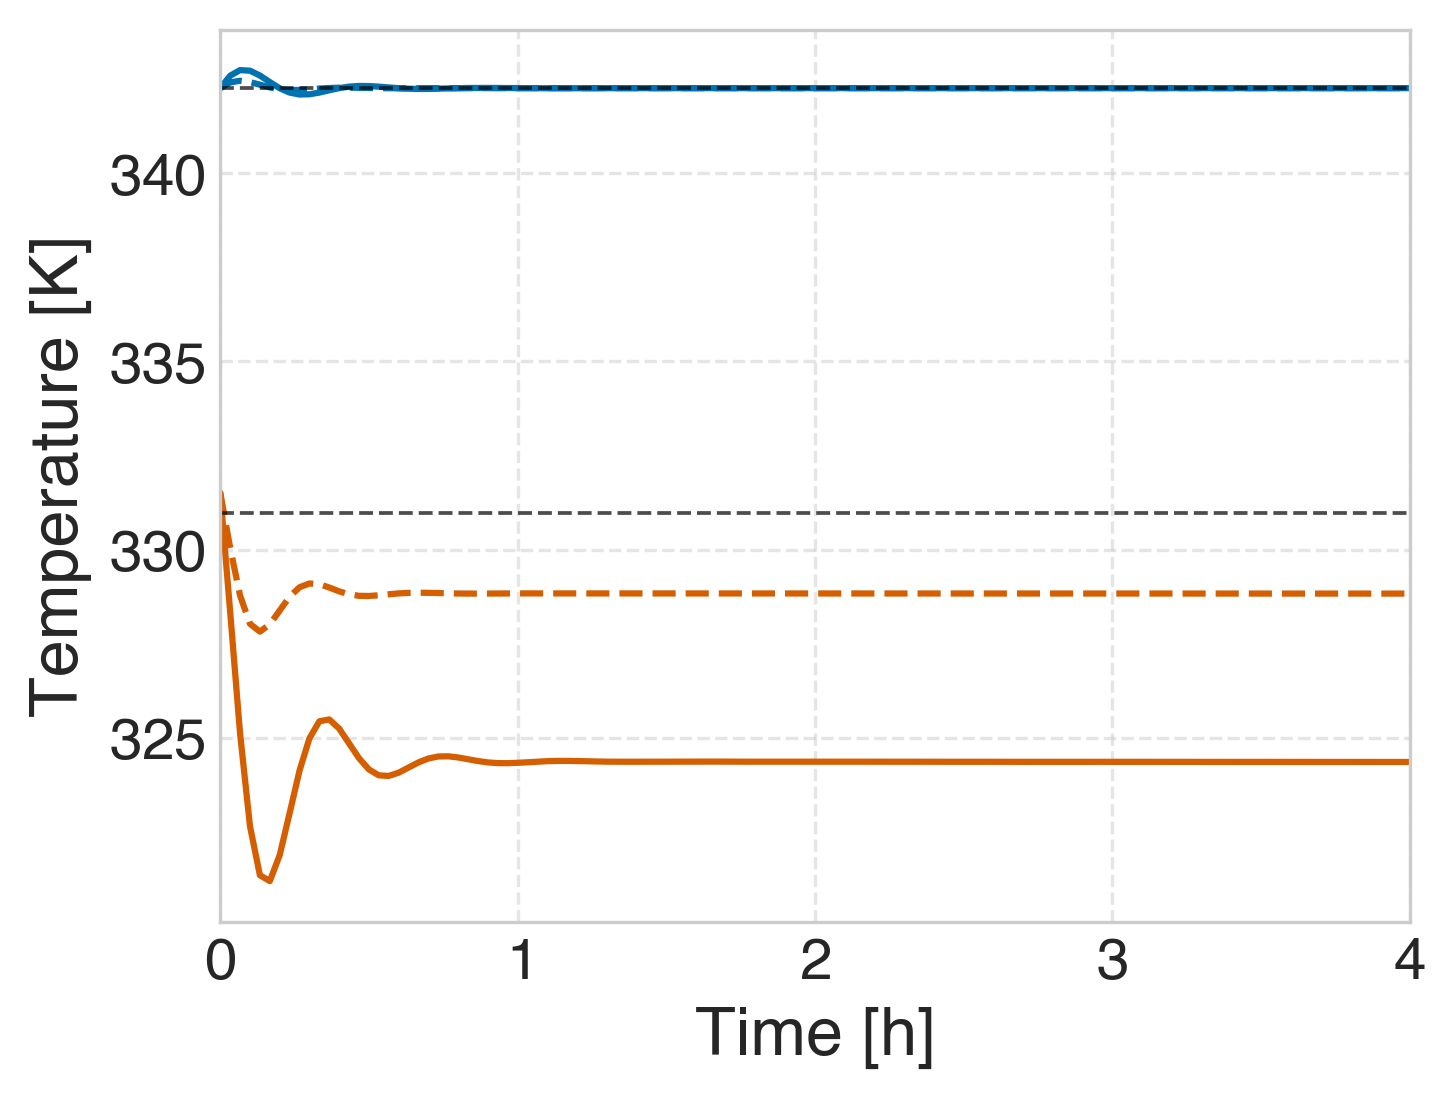
\includegraphics[width=0.9\linewidth]{nb21_cl_vs_ol_masking_2x1}
  \caption{Control masking in System~II under jacket fouling
    (noiseless). W5: $\beta_r=0.80$, dashed lines; W6: $\beta_r=0.60$, full lines. 
    Reactor temperature $T_r$ is shown in blue, jacket temperature $T_j$ in orange.
    Reactor temperature stays near the setpoint
    (dashed black line) under closed-loop operation regardless of fouling severity as Loop~1 masks the fault in the temperature channel. Jacket temperature $T_j$ drops proportionally to the
    fouling magnitude, providing
    the primary secondary observable for $\beta_r$.}
  \label{fig:wu_cl_masking}
\end{figure}
% ------------------------------------------------------------------

\subsection{Fault Scenarios and Parameterisation}
\label{sec:fault_params2}

Five independent multiplicative degradation factors are inferred from process observations (Table~\ref{tab:wu_fault_params}). The two reactor-side parameters ($\alpha$, $\beta_r$) from System~I plus three parameters to capture column and feed degradation: $\eta_\mathrm{col}$, $\xi_\mathrm{reb}$,  and $z_{A0,\mathrm{eff}}$. The first four parameters are multiplicative factors on the nominal physical constants, while $z_{A0,\mathrm{eff}}$ is an effective fresh-feed A fraction that accounts for variability
in the feed composition or upstream separation efficiency. The lower bound $\eta_\mathrm{col} \geq 0.80$ is imposed by numerical stability of the quasi-steady-state column shortcut.

% ------------------------------------------------------------------
\begin{table*}[tb]
\centering
\caption{Fault parameters for System~II (Wu 2003 recycle plant). All parameters
  equal 1.0 at clean-service nominal conditions. The physical design constants
  $U\!A_r$ and $U\!A_\mathrm{reb}$ are treated as known and only the relative
  degradation factors are inferred.}
\label{tab:wu_fault_params}
\small
\begin{tabular}{clll}
\toprule
Symbol & Physical meaning & Prior & Primary observable \\  
\midrule
$\alpha$ & Catalyst activity factor & $\mathcal{U}(0.4,\,1.2)$ & $F_{R,\mathrm{norm}}$, $Q_j$ \\
$\beta_r$ & Reactor jacket conductance factor & $\mathcal{U}(0.4,\,1.2)$ & $T_j$, $Q_j$ \\
$\eta_\mathrm{col}$ & Empirical column separation factor & $\mathcal{U}(0.80,\,1.0)$ & $T_\mathrm{reb}$, $Q_\mathrm{reb}$ \\
$\xi_\mathrm{reb}$ & Reboiler conductance factor & $\mathcal{U}(0.4,\,1.2)$ & $Q_\mathrm{reb}$ \\
$z_{A0,\mathrm{eff}}$ & Effective fresh-feed A fraction & $\mathcal{U}(0.70,\,0.95)$ & All channels via reactor SS \\
\bottomrule
\end{tabular}
\end{table*}
% ------------------------------------------------------------------

Incorporating all five degradation factors, the complete reactor--column--recycle
model replaces Eqs.~\eqref{eq:wu_reactor} and \eqref{eq:wu_recycle} with
%
\begin{subequations}
\label{eq:wu_degraded}
\begin{align}
  \frac{dz_A}{dt}
    =& \frac{F_\mathrm{in}}{M_r}\bigl(z_{A,\mathrm{in}} - z_A\bigr)
       - \alpha\,k(T_r)\,z_A,
  \label{eq:wu_dza_degraded} \\[4pt]
  \frac{dT_r}{dt}
    =& \frac{F_\mathrm{in}}{M_r}\bigl(T_\mathrm{in,mix} - T_r\bigr)
       + \frac{-\Delta H_r}{\rho C_p}\,\alpha\,k(T_r)\,z_A \nonumber \\
     & - \frac{\beta_r\,U\!A_r}{\rho C_p V_r}\bigl(T_r - T_j\bigr),
  \label{eq:wu_dtr_degraded} \\[4pt]
  \frac{dT_j}{dt}
    =& \frac{\beta_r U\!A_r(T_r - T_j) - Q_j}{M_j\,C_{pj}},
  \label{eq:wu_dtj_degraded}
\end{align}
\end{subequations}
%
where the fresh-feed composition fault propagates through the feed-mixing relation
%
\begin{equation*}
  z_{A,\mathrm{in}} = \frac{F_0\,z_{A0,\mathrm{eff}} + F_R\,x_D}{F_\mathrm{in}},
  \qquad
  T_\mathrm{in,mix} = \frac{F_0\,T_\mathrm{in} + F_R\,T_r}{F_\mathrm{in}},
  \label{eq:wu_zain_degraded}
\end{equation*}
%
replacing the healthy-feed value $z_0 = 0.90$ of Eq.~\eqref{eq:wu_recycle} by the inferred effective composition $z_{A0,\mathrm{eff}}$.  The empirical column separation
factor $\eta_\mathrm{col}$ scales the effective relative volatility away from its clean-service value, Eq.~\eqref{eq:wu_alphaeff},
%
\begin{equation}
  \alpha_\mathrm{eff} = 1 + \eta_\mathrm{col}\,(\alpha_\mathrm{rel} - 1),
  \label{eq:wu_alphaeff_degraded}
\end{equation}
%
which sets $x_D$, $x_B$, and hence the recycle flow $F_R$ appearing in Eqs.~\eqref{eq:wu_dza_degraded} and \eqref{eq:wu_zain_degraded}.  Finally, the
reboiler conductance factor $\xi_\mathrm{reb}$ scales the heat duty that Loop~3 must 
supply to hold the
column material balance at its quasi-steady state. 
The nominal column operating point ($x_{B,\mathrm{nom}}$, $F_{\mathrm{in,nom}}$, and the clean-service
boilup reference) is taken from the Wu benchmark~\citep{Wu2003}, while the following algebraic duty relation
is an empirical quasi-steady proxy. 
Its form encodes four effects: nominal duty scales with throughput $F_\mathrm{in}/F_{\mathrm{in,nom}}$, 
with the boilup command $V_\mathrm{norm}$ from Loop~3, inversely with reboiler conductance 
$\xi_\mathrm{reb}$, and upward with bottoms impurity $(x_B-x_{B,\mathrm{nom}})$ 
and column-separation loss $(1-\eta_\mathrm{col})$,
%
\begin{equation}
  \begin{aligned}
  Q_\mathrm{reb} ={}& \frac{Q_{\mathrm{reb,nom}}}{\xi_\mathrm{reb}}
    \frac{F_\mathrm{in}}{F_{\mathrm{in,nom}}} V_\mathrm{norm} \\
    &\times \left[1 + 2\,(x_B - x_{B,\mathrm{nom}}) + 0.5\,(1 - \eta_\mathrm{col})\right],
  \end{aligned}
  \label{eq:wu_qreb_degraded}
\end{equation}
%
where $F_{\mathrm{in,nom}} = F_0 + F_{R,\mathrm{nom}}$, $x_{B,\mathrm{nom}}=0.011$, and $V_\mathrm{norm}$ is the normalised boilup effort commanded by Loop~3. A fouled reboiler ($\xi_\mathrm{reb} < 1$) therefore requires a proportionally larger duty $Q_\mathrm{reb}$ for the same throughput and boilup effort which is directly analogous to the role of $\beta_r$ in the reactor jacket balance, Eq.~\eqref{eq:wu_dtj_degraded}.

Table~\ref{tab:si_wu_scenarios} lists the fourteen closed-loop fault scenarios studied through 30 stochastic replicates each giving rise to 420 observation windows. The scenarios cover individual single-parameter faults, compound multi-parameter faults, and a near-snowball-tipping-point scenario.  
%Full scenario definitions are provided in Table~S2 of the Supporting Information.
Data generation follows the same Euler--Maruyama protocol as System~I, adapted to 2-hour windows at 1-min sampling resolution (120 time steps). The process-noise levels and training hyperparameters are detailed in Section~S7 of the Supporting Information.

% ------------------------------------------------------------------
\begin{table*}[tb]
\centering
\caption{Fault scenario catalogue for System~II. All scenarios use 30 independent
  stochastic replicates per control structure, each comprising a 2-hour observation
  window at 1-min sample interval (120 time steps). Parameters equal 1.0 unless
  otherwise listed.}
\label{tab:si_wu_scenarios}
\small
\begin{tabular}{cllcccccl}
\toprule
ID & Name & Fault unit & $\alpha$ & $\beta_r$ & $\eta_\mathrm{col}$ & $\xi_\mathrm{reb}$ & $z_{A0}$ & Primary purpose \\
\midrule
W1  & Healthy nominal     & Healthy  & 1.00 & 1.00 & 1.00 & 1.00 & 0.90 & SBI training / baseline \\
W2  & Cat.~decay mild     & Reactor  & 0.85 & 1.00 & 1.00 & 1.00 & 0.90 & Single-param: $\alpha$ \\
W3  & Cat.~decay severe   & Reactor  & 0.65 & 1.00 & 1.00 & 1.00 & 0.90 & Snowball onset \\
W4  & Cat.~near tipping   & Reactor  & 0.55 & 1.00 & 1.00 & 1.00 & 0.90 & Near snowball limit \\
W5  & Jacket fouling mild & Reactor  & 1.00 & 0.80 & 1.00 & 1.00 & 0.90 & Single-param: $\beta_r$ \\
W6  & Jacket fouling severe& Reactor & 1.00 & 0.60 & 1.00 & 1.00 & 0.90 & Single-param: $\beta_r$ \\
W7  & Col.~sep.~loss      & Column   & 1.00 & 1.00 & 0.80 & 1.00 & 0.90 & Single-param: $\eta_\mathrm{col}$ \\
W9  & Reboiler fouling    & Column   & 1.00 & 1.00 & 1.00 & 0.70 & 0.90 & Single-param: $\xi_\mathrm{reb}$ \\
W10 & Feed purity drop    & Feed     & 1.00 & 1.00 & 1.00 & 1.00 & 0.78 & Single-param: $z_{A0}$ \\
W11 & Cat.~+ jacket       & Reactor  & 0.80 & 0.80 & 1.00 & 1.00 & 0.90 & Compound: reactor faults \\
W12 & Cat.~+ col.~sep.    & Multi    & 0.75 & 1.00 & 0.80 & 1.00 & 0.90 & Compound: cross-unit \\
W13 & Cat.~+ feed         & Multi    & 0.80 & 1.00 & 1.00 & 1.00 & 0.80 & Compound: reactor + feed \\
W15 & Cat.~near tipping   & Reactor  & 0.58 & 1.00 & 0.90 & 1.00 & 0.90 & Near snowball tipping \\
W16 & Full multi-fault    & Multi    & 0.75 & 0.80 & 0.80 & 0.85 & 0.90 & All-unit degradation \\
\bottomrule
\end{tabular}
\end{table*}
% ------------------------------------------------------------------

% =============================================================================
\section{Inference Methodology}\label{sec:methodology}
% =============================================================================

The inference framework applied in this work is known as \emph{simulation-based inference} (SBI), a likelihood-free inference methodology used when the likelihood function $p(\mathbf{y} \mid \boldsymbol{\theta})$ is analytically intractable or unavailable, but simulation of synthetic data $\mathbf{y}_\text{sim} \sim p(\mathbf{y} \mid \boldsymbol{\theta})$ is feasible \citep{Cranmer2020}. 
This methodology is widely used in scientific applications where the underlying physical model is known, but the complexity of the system makes it difficult to derive a closed-form expression for the likelihood
%(Section~\ref{sec:related_work} positions this work against the one prior
%application of SBI to chemical-process equipment monitoring, \citet{Collett2026}).
In such cases, SBI allows for the estimation of posterior distributions over model parameters by leveraging simulations to generate synthetic datasets that can be compared to observed data. This is the case for the closed-loop fault-diagnosis 
problem considered here: the simulator includes nonlinear process dynamics,
feedback control, stochastic disturbances, and sensor noise, while the likelihood
of the resulting window-level summaries is not analytically tractable.
The applied SBI framework comprises three successive stages: (i)~A JAX-vectorised stochastic simulator that generates synthetic observation windows from the degraded closed-loop models. (ii)~An amortised neural posterior estimator trained to approximate the Bayesian posterior $p(\boldsymbol{\theta}\mid\mathbf{s})$ over the degradation-parameter vector $\boldsymbol{\theta}$ given any realisation of the summary statistics. (iii)~A threshold-and-unit-aggregation rule (Section~\ref{sec:fault_class}) that maps the joint posterior to a discrete fault class, reducing to four non-overlapping quadrants of the fault-parameter space for System~I and to five unit-level classes for System~II. 
The inference methodology is identical across System~I (Section~\ref{sec:system1}) and System~II
(Section~\ref{sec:system2}) and differs only in the dimensionality of $\boldsymbol{\theta}$, the summary statistics $\mathbf{s}$, and the density-estimator training configuration (hyperparameters).
The framework is implemented in the \texttt{sbi} library~\citep{Tejero_cantero_3be1efca,BoeltsDeistler_sbi_2025}.
Following the notation of \citet{Cranmer2020}, the estimator is operated in the \emph{amortised} regime: the simulator is only queried at training time, and subsequent
inference on any new 60-minute window requires only a single forward pass through the trained network, with typical latency below 20~ms.
%The three stages are described in detail below.


\subsection{Amortised Posterior Estimation and Classification}
\label{sec:sbi_method}
% ---------------------------------------------------------------------------

%\subsubsection{Prior distribution and inference target}
The inference target is an $n$-dimensional degradation-parameter vector $\boldsymbol{\theta}=(\theta_1,\ldots,\theta_n)$, with each component
assigned an independent uniform prior distribution:
%
\begin{equation}
  p(\boldsymbol{\theta}) =
  \bigotimes_{j=1}^{n}
  \mathcal{U}\!\bigl([\theta_{j,\mathrm{lo}},\,\theta_{j,\mathrm{hi}}]\bigr).
  \label{eq:prior}
\end{equation}
%
For System~I, $n=2$ and $\boldsymbol{\theta}=(\alpha,\beta)$, both assigned
$\mathcal{U}(0.4,\,1.2)$ (Table~\ref{tab:params_system1}). For System~II,
$n=5$ and
$\boldsymbol{\theta}=(\alpha,\beta_r,\eta_\mathrm{col},\xi_\mathrm{reb},z_{A0,\mathrm{eff}})$,
with per-parameter bounds given in Table~\ref{tab:wu_fault_params}.
For the parameters shared across both systems which are centred on a healthy value of 1 ($\alpha$; $\beta$ or $\beta_r$; $\xi_\mathrm{reb}$), the upper bound of 1.2 serves dual purpose: it allows for a small positive bias in the estimated parameters, and it provides a numerical buffer around the healthy operating point, preventing the density estimator from being trained against a hard boundary at the most frequently sampled condition. The remaining two System~II parameters have bounds set by other constraints (Table~\ref{tab:wu_fault_params}): $\eta_\mathrm{col}$'s lower bound of 0.80 is set by the numerical stability of the quasi-steady-state column shortcut (Section~\ref{sec:fault_params2}), and $z_{A0,\mathrm{eff}}$'s bounds are centred on its own healthy value of 0.90, not 1.

A conditional density estimator $q_\phi(\boldsymbol{\theta}\mid\mathbf{s})$ is trained by minimising the expected forward Kullback--Leibler divergence over simulated $(\boldsymbol{\theta},\mathbf{s})$ pairs drawn from the joint prior-predictive distribution,
%
\begin{equation}
  \mathcal{L}(\phi)
  \;=\;
  -\,\mathbb{E}_{p(\boldsymbol{\theta})\,p(\mathbf{y}\mid\boldsymbol{\theta})}
  \!\Bigl[
    \log q_\phi\!\bigl(\boldsymbol{\theta}\mid\mathbf{s}(\mathbf{y})\bigr)
  \Bigr].
  \label{eq:snpe_loss}
\end{equation}
%
Here, $\mathbf{s}(\mathbf{y})$ is the summary-statistic vector extracted from the raw observation window $\mathbf{y}$, and $p(\mathbf{y}\mid\boldsymbol{\theta})$ 
is the stochastic simulator (Section~\ref{sec:scenarios}). The expectation is 
approximated by Monte Carlo sampling of $(\boldsymbol{\theta},\mathbf{y})$ pairs 
from the prior and simulator, and the loss is minimised with respect to the density-
estimator parameters $\phi$ using stochastic gradient descent. 
The trained estimator $q_\phi$ thus approximates $p(\boldsymbol{\theta}\mid\mathbf{s})$ for summary statistics reachable under the prior predictive distribution, enabling deployment on new observation windows without retraining.
This is the single-round amortised formulation of sequential neural posterior estimation~\citep[SNPE-C;][]{Greenberg2019}, in which the proposal distribution coincides with the prior so that no importance correction is required.  

%\paragraph{Relation to the direct method of closed-loop identification.}
Following \citet{Forssell1999}, SNPE-C operates on the measured signal histories $\mathbf{x}(t)$ without requiring an explicit model of the feedback controller, making it a probabilistic analogue of the \emph{direct method} of closed-loop system identification. Like the classical direct approach, it is universally applicable to nonlinear and
saturating feedback and exploits the persistent in-loop process noise to partially recover parameter information that is structurally reduced by integral action~\citep{Ljung1999}.

The conditional distribution $q_\phi(\theta\vert{}s)$ is parameterised by a neural spline flow~\citep{Durkan2019}. 
Network architectures, training budgets ($n_{sim} = 10,000$ for System I; $15,000$
for System II), and ensembling strategies were selected to obtain stable posterior 
estimates and acceptable calibration for the downstream diagnostic task.
Full details of the network architectures, hyperparameter sweeps, and seed-stability strategies are 
provided in the Supporting Information (Sections S3 and S7.3). The Supporting Information also gives the exact simulation, summary-statistic, and calibration protocols used to reproduce the reported tables and figures.

Posterior calibration is assessed using simulation-based calibration~\citep{Talts2018}, 
which tests whether the rank of the true parameter among posterior draws is uniformly
distributed across independent test cases drawn from the prior. 
The full protocol, acceptance criteria, and rank histograms for each system's production posterior are
given in the Supporting Information (Section~S6, System~I; Section~S9.2, System~II).

\phantomsection\label{sec:fault_class}
The joint posterior $q_\phi(\boldsymbol{\theta}\mid\mathbf{s})$ is mapped 
to a discrete fault class by a two-level rule applied to both systems, though
the per-parameter threshold value now differs between them. First, each
degradation parameter $\theta_j$ is compared against a relative threshold
$\theta_\mathrm{thr}$ and flagged as degraded if $\theta_j<\theta_\mathrm{thr}$. 
For System~II, $\theta_\mathrm{thr}=0.85$ (a 15\% reduction relative to clean-service
baseline) for the reactor- and column-side parameters ($\alpha$, $\beta_r$, 
$\eta_\mathrm{col}$, $\xi_\mathrm{reb}$), exceeding typical run-to-run variability
and providing a meaningful trigger for maintenance decisions; $z_{A0,\mathrm{eff}}$
is flagged relative to its own healthy value of 0.90, since a feed-purity fault is
one-sided (always a reduction, never an increase), flagging a compositional deviation
rather than a rate-constant or heat-transfer-coefficient reduction. For System~I, 
$\theta_\mathrm{thr}=0.90$ for both $\alpha$ and $\beta$. This threshold defines
the operational fault-class decision rule and does not affect the posterior
parameter estimates. Scenarios close to the threshold should therefore be
interpreted as tests of both posterior uncertainty and the chosen decision rule.\\
Second, parameters are grouped into physical units such
that for System~I, each of the two parameters is its own unit; while for System~II, 
reactor $=\{\alpha,\beta_r\}$, column $=\{\eta_\mathrm{col},\xi_\mathrm{reb}\}$, 
feed $=\{z_{A0,\mathrm{eff}}\}$. A unit is flagged degraded if any of its member 
parameters is degraded. The reported class is the combination of degraded units with 
the greatest posterior mass: \emph{healthy} (no unit degraded), the corresponding 
unit label if exactly one unit is degraded, or \emph{multi} 
if more than one unit is degraded simultaneously. The associated confidence is given
by the posterior mass assigned to the reported class. For System~I, with 
two parameters each forming its own unit, this reduces to four non-overlapping
quadrants of the $(\alpha,\beta)$ plane: \emph{healthy}, \emph{fouling-dominant},
\emph{decay-dominant}, and \emph{multi}. For System~II it produces five classes 
(healthy, reactor, column, feed, multi), detailed in Section~\ref{sec:wu_fault_class}.
For the feed parameter this posterior-decision rule corresponds to
$z_{A0,\mathrm{eff}} < 0.85\times0.90 = 0.765$. This posterior-decision threshold is
distinct from the scenario-design labels in Table~\ref{tab:si_wu_scenarios}, which 
define the intended fault unit of each synthetic case before posterior classification is applied.

% =============================================================================
\section{Results: System~I --- Propylene Oxide CSTR}
\label{sec:results_system1}
% =============================================================================

% ---------------------------------------------------------------------------
%\subsection{Physics-Informed Summary Statistics}
%\label{sec:summary_stats}
% ---------------------------------------------------------------------------

% ---------------------------------------------------------------------------
\subsection{Model Validation and Fault Classification}
\label{sec:snapshot_classification}
% ---------------------------------------------------------------------------

Each replicate observation window $\mathbf{x}\in\mathbb{R}^{120\times4}$ is 
compressed to a 29-dimensional
summary-statistic vector $\mathbf{s}(\mathbf{x})\in\mathbb{R}^{29}$ before inference. 
Most entries are
generic time-series and control-effort descriptors (Table~S1), 
while two are physics-informed proxies:
%
\begin{align}
  s_{U\!A} &= \frac{\bar{T}-\bar{T}_c}{\bar{Q}_c},
  \label{eq:ua_proxy}\\[4pt]
  s_{k_0} &= \ln\!\left(\frac{\bar{C}}{C_i - \bar{C}}\right),
  \label{eq:k0_proxy}
\end{align}
where $\bar{(\cdot)}$ denotes the whole-window mean.
The feature $s_{U\!A}$ is a conductance-sensitive descriptor: 
lower effective heat transfer generally requires a larger temperature
difference per unit coolant effort. Analogously, the feature $s_{k_0}$ is
motivated by the component balance:
\begin{equation} 
  s_{k_0} = \ln(Q/V)-\ln\alpha-\ln k(T), 
  \label{eq:k0_proxy_interpretation} 
\end{equation}
to be a simplified reaction-rate-sensitive proxy.

% ------------------------------------------------------------------
\begin{figure}[tb]
  \centering
  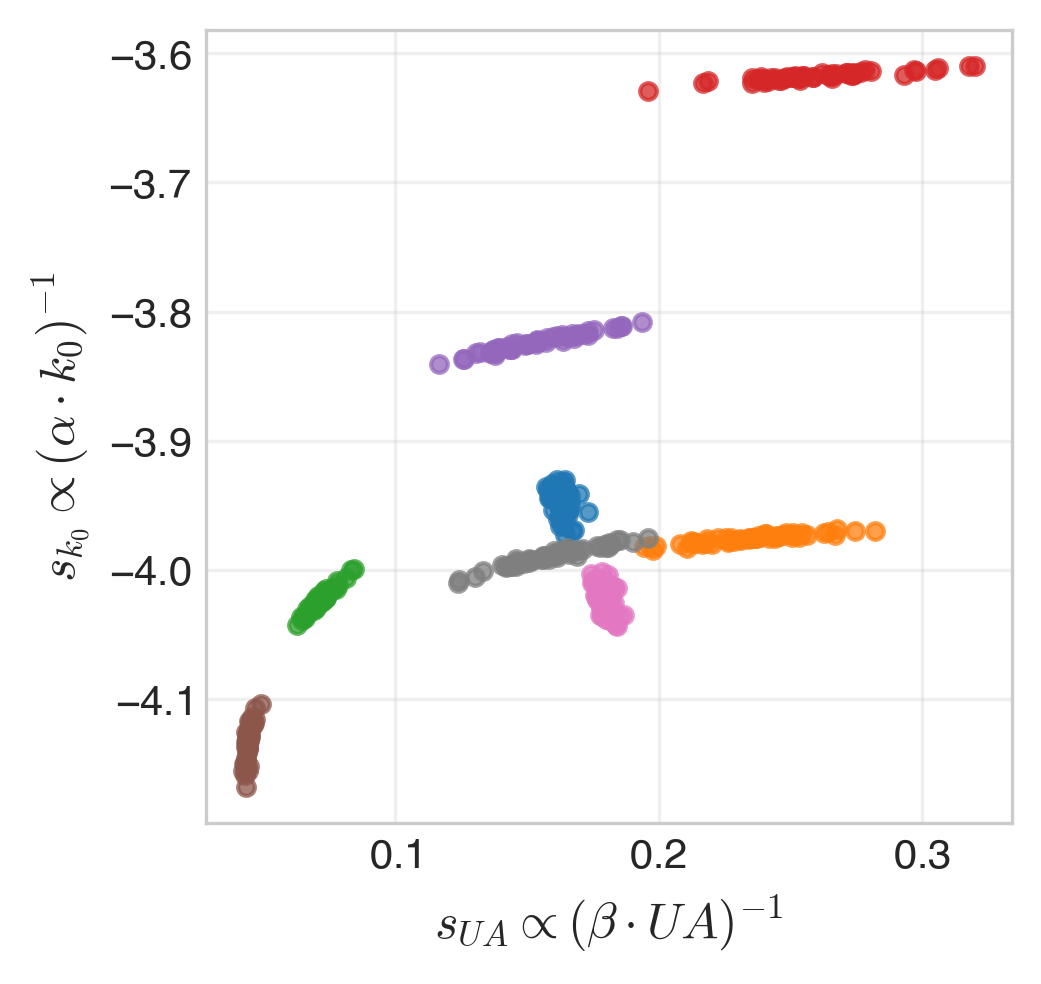
\includegraphics[width=0.85\linewidth]{03_physics_features_scatter}
  \caption{Scenario separation in the two physics-informed summary
    features. Each point represents one of the 50 stochastic
    replicates with colour indicating scenario (Sc0-Sc7). The $x$-axis encodes
    $s_{U\!A} \propto (\beta\!\cdot\!U\!A)^{-1}$, the $y$-axis encodes
    $s_{k_0} \propto (\alpha\!\cdot\!k_0)^{-1}$. Closed loop 
    scenarios (Sc1-Sc5) appear as thin strands while open-loop scenarios 
    (Sc0, Sc6) are more clustered. Scatter within
    each cluster is due to process and sensor noise.}
  \label{fig:physics_scatter}
\end{figure}
% ------------------------------------------------------------------

Simulator coverage of the evaluation regime was confirmed through prior predictive
checks over 500 parameter vectors drawn from the prior, spanning the observed data
range for all 29 summary features across every closed-loop scenario ~\citep{Cranmer2020} 
(Fig.~S1 of the Supporting
Information). Posterior calibration with 500 test cases, drawn and evaluated under
the matched (scenario-specific warm-start) protocol used throughout, does not reject
rank uniformity at the 5\% level (Kolmogorov-Smirnov (KS) $p$-values of $0.21$ for
$\alpha$ and $0.13$ for $\beta$; two-sample classifier scores of 0.53 and 0.52,
close to the uninformative baseline of 0.5). Rank histograms, SBC implementation
details, and the matched-protocol calibration interpretation are given in
Supporting Information Section~S6.
%
\begin{figure}[tb]
  \centering
%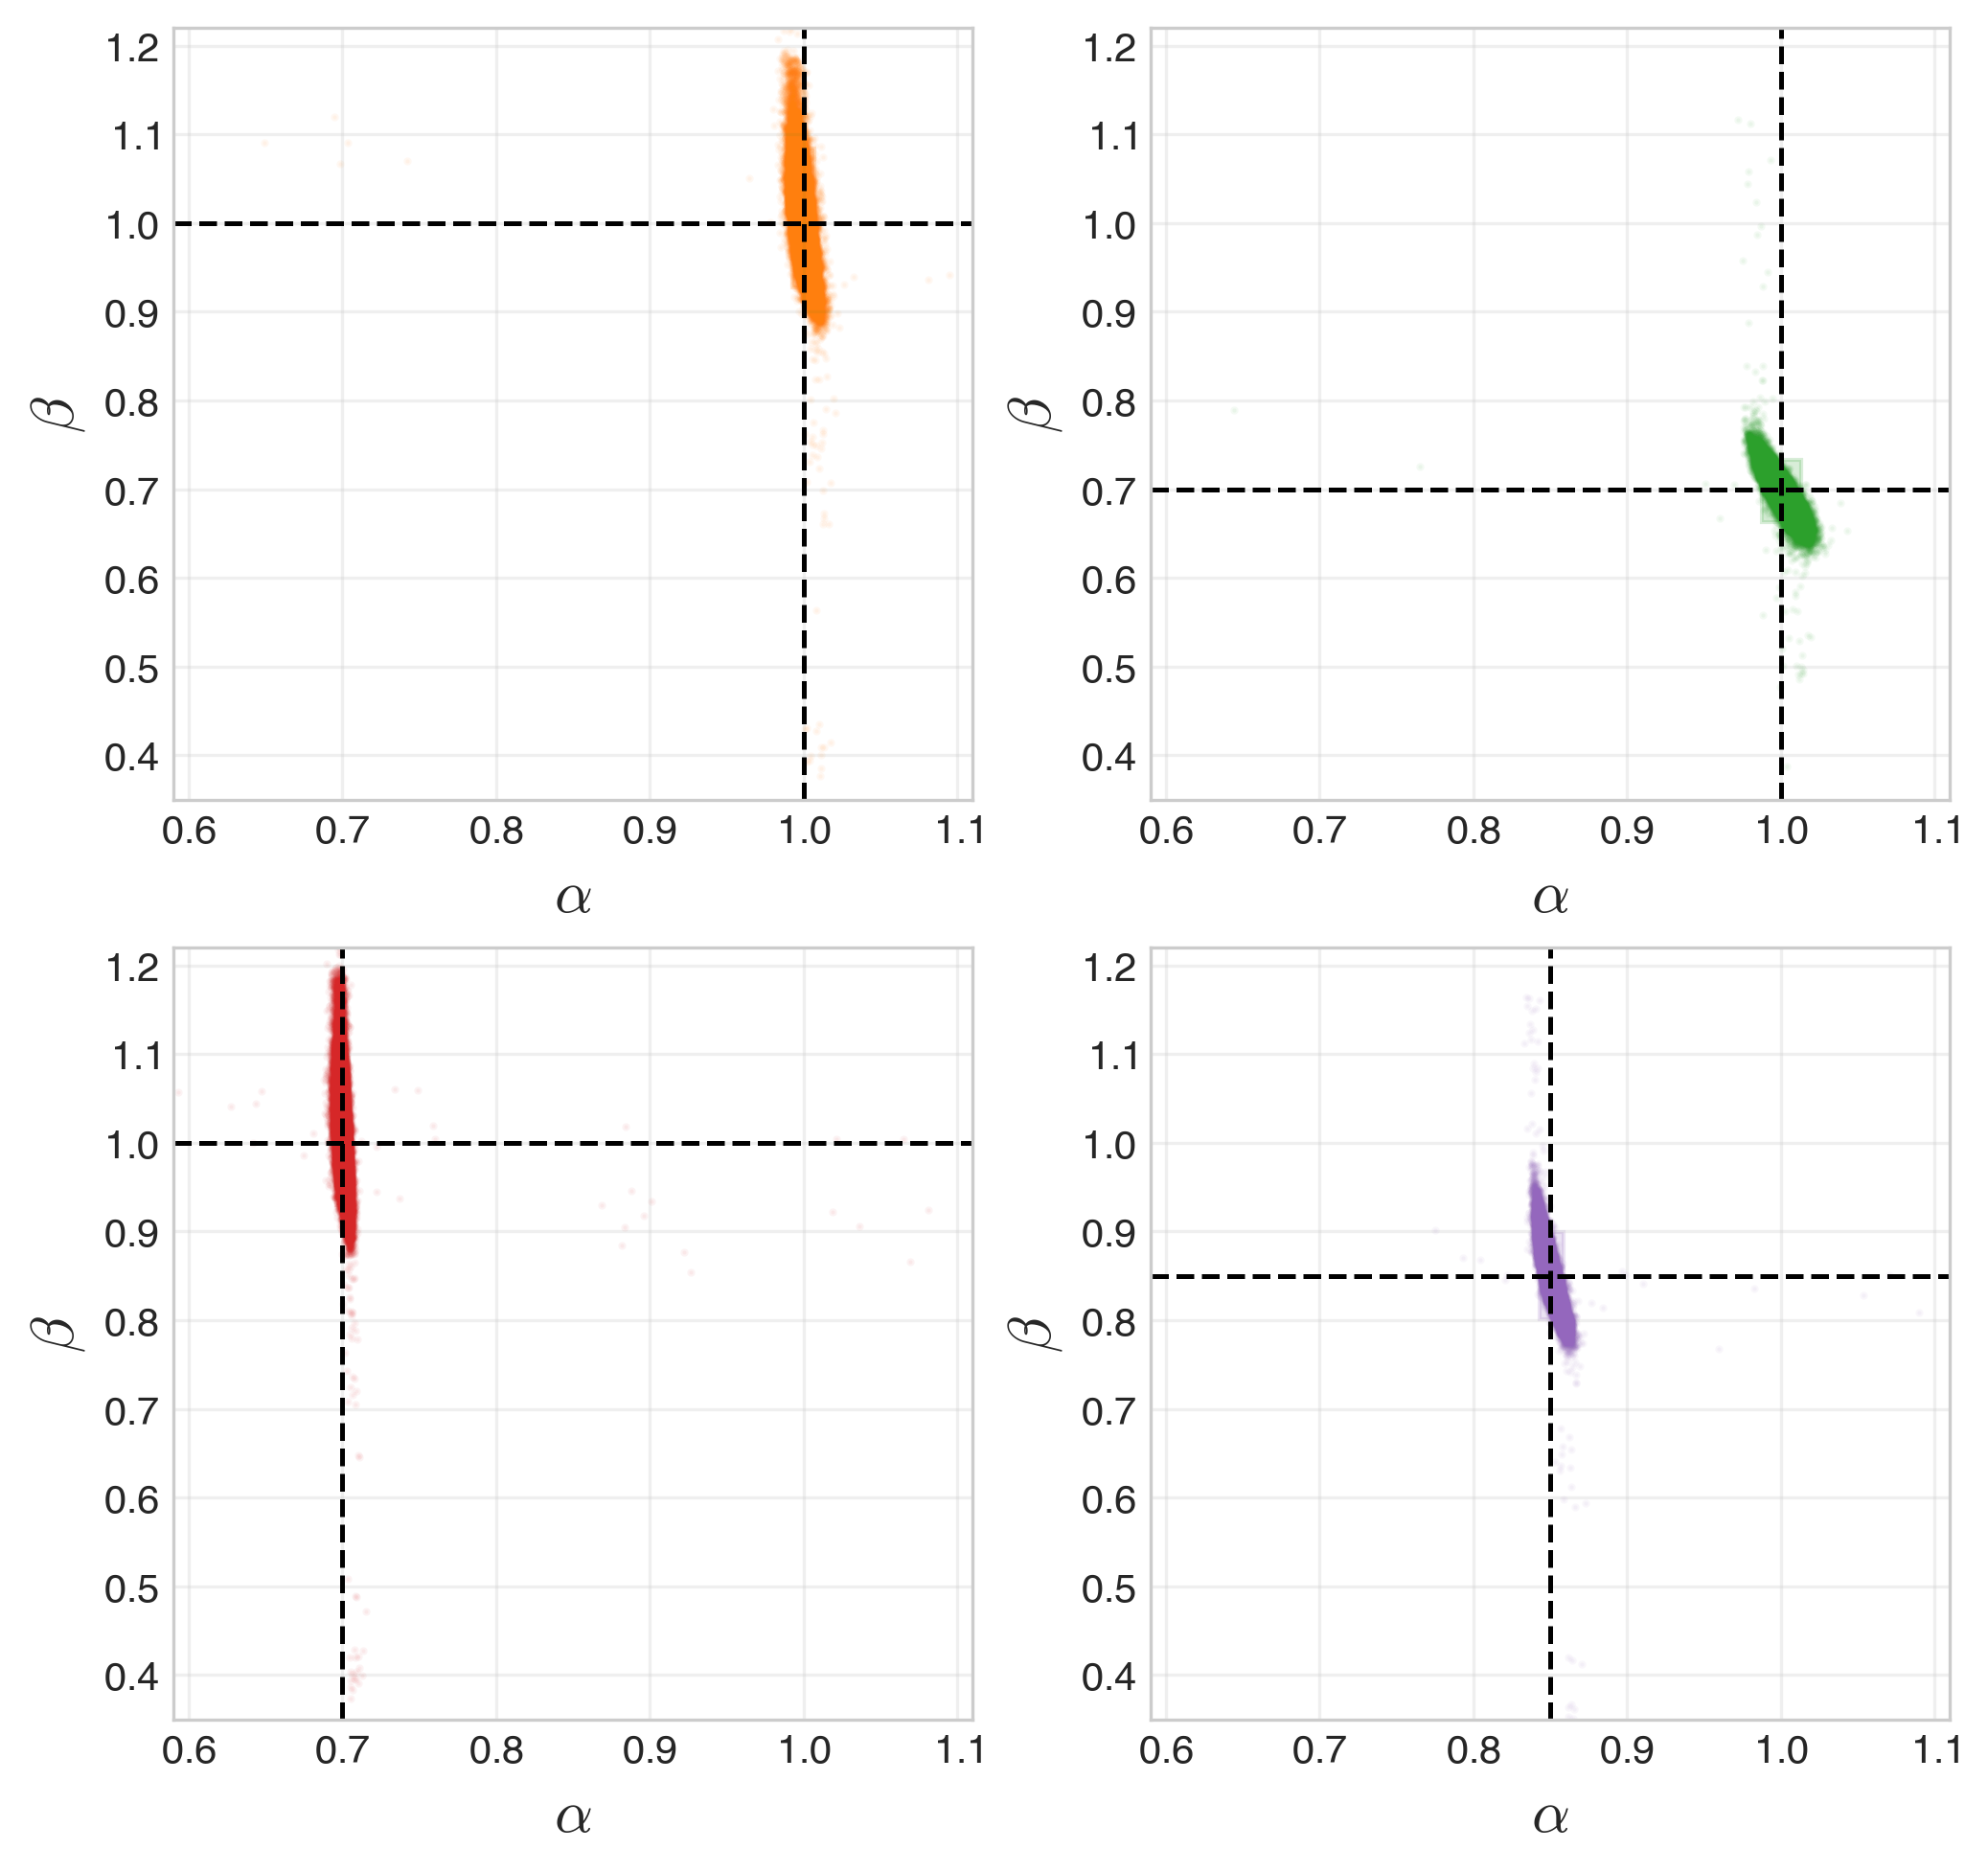
\includegraphics[width=0.95\linewidth]{06_joint_posterior_primary.png}
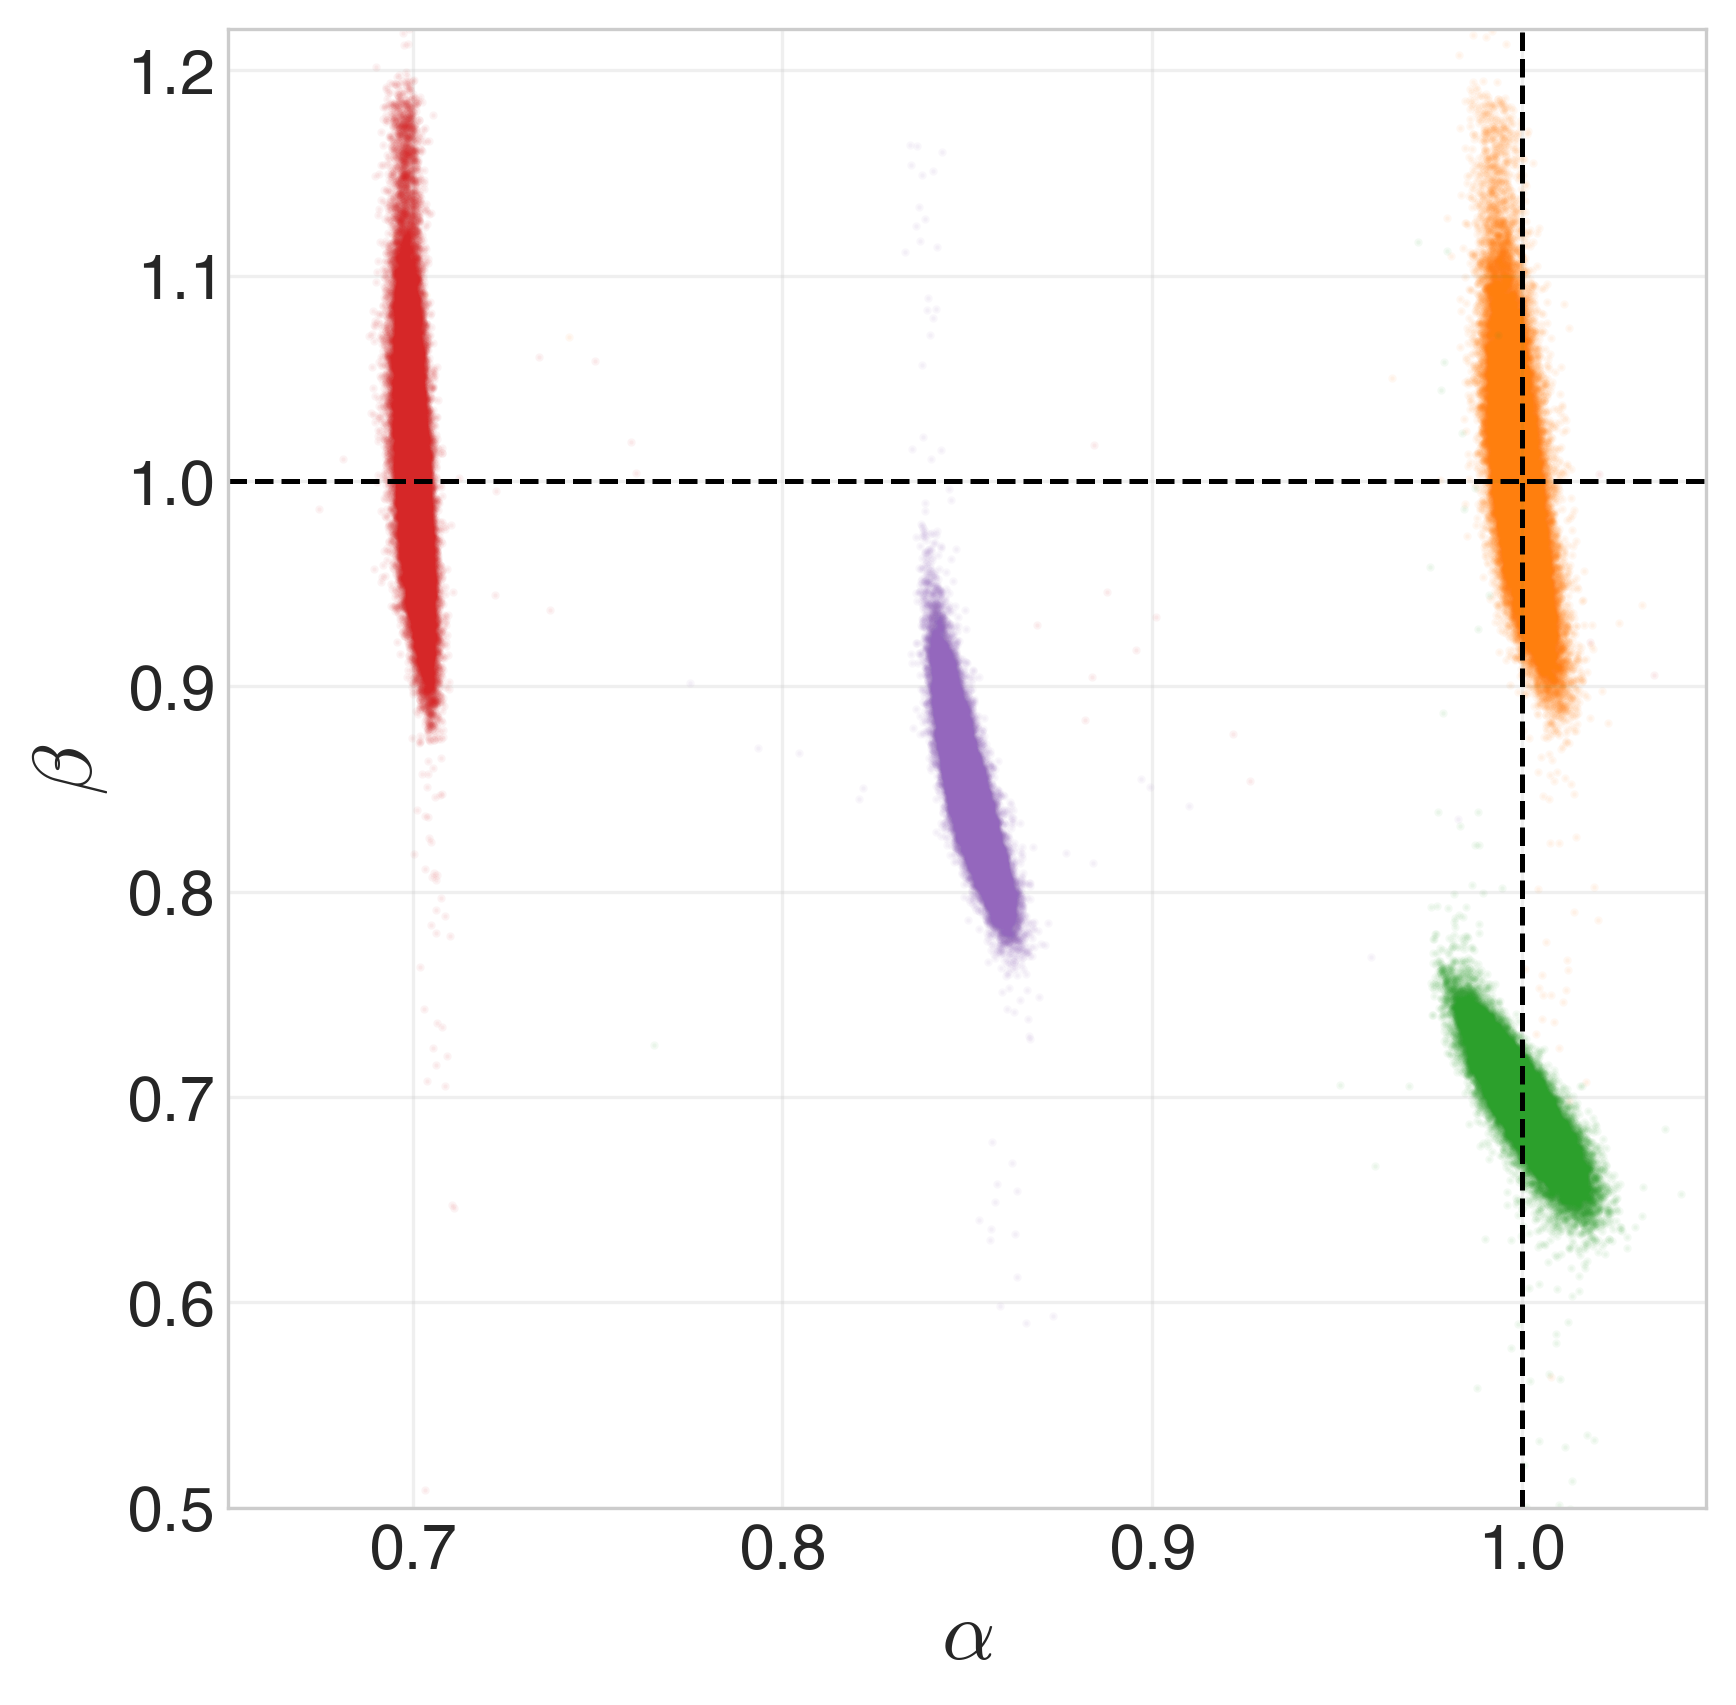
\includegraphics[width=0.8\linewidth]{06_joint_posterior_primary_merged}
  \caption{Joint posterior samples for the primary System I closed loop scenarios: Sc1 (normal operation,
  orange), Sc2 (fouling, green), Sc3 (catalyst decay, red), Sc4 (combined, purple). 
  Each panel pools posterior samples for one scenario and plots the inferred degradation
  parameters $\alpha$ and $\beta$. 
  Dashed black lines mark the true scenario values. The narrow vertical structure of the posteriors
  indicates that $\alpha$ is generally tightly constrained, 
  while $\beta$ varies more strongly across the fault scenarios.}\label{fig:posterior_recovery}
\end{figure}
We evaluate fault separability in two complementary ways. First, as a diagnostic
check on the summary representation, we train a supervised Linear Discriminant
Analysis (LDA) classifier on the simulated scenario labels~\citep{Zhou2021}. This
tests whether the summaries contain enough information to separate the known
fault classes. Second, for the SBI posterior itself, fault classes are assigned
without historical labelled plant faults by applying the posterior threshold rule
defined in Section~\ref{sec:fault_class}.

The two-feature $\{s_{U\!A},\,s_{k_0}\}$ proxy set was found to be sufficient for
near-perfect closed-loop LDA classification (99.3\% accuracy; macro-$F_1=0.993$), as expected from 
Figure~\ref{fig:physics_scatter}. The full
29-feature set removed the remaining boundary errors, giving perfect LDA classification for both
closed- and open-loop scenarios. Separately, mapping SBI posterior samples to the four
threshold-defined fault regions gave a closed-loop macro-F\textsubscript{1} of
0.927 (Table~\ref{tab:scenario_results}).
Coverage (90$\%$ of confidence interval) 
is close to its nominal level for the non-saturating matched closed-loop scenarios,
but falls to 0.62 for Sc5. In this severe-fouling case, the coolant actuator is saturated for a
substantial fraction of each window, reducing sensitivity to further changes in $\beta$ and 
producing under-dispersed marginal intervals.
The lower score for Sc\,7 is due to a genuine confound between the temperature-measurement
bias and the $\beta$ degradation, which pulls the posterior mean upward toward the 0.90 classification
threshold. This is a confound between the effect of the fault and the effect of the biased measurement channel. 

% ------------------------------------------------------------------
\begin{table}[tb]
\centering
\caption{System~I per-scenario evaluation results for the production NSF
  posterior (50 replicates per scenario).  $\hat{\alpha}$
  and $\hat{\beta}$ are posterior means, 90\%~CI coverage gives the
  fraction of replicates for which the 90\% credible interval contains
  the true value, $F_1$ is the per-scenario fault-classification F\textsubscript{1}
  score.  Open-loop scenarios (Sc\,0, Sc\,6) are evaluated with a
  closed-loop-trained posterior and therefore reflect the mode-mismatch
  penalty discussed in Section~\ref{sec:model_mismatch_results}. 
  The $+2$~K temperature-measurement bias pulls $\hat\beta$ upward toward the
  $0.90$ classification boundary; this is a genuine measurement-bias/fault confound.}
\label{tab:scenario_results}
\small
\begin{tabular}{clccrrrr}
\toprule
ID & Name & $\alpha^*$ & $\beta^*$ &
$\hat{\alpha}$ & $\hat{\beta}$ & CI %$\beta$ 
& $F_1$ \\
\midrule
Sc\,0 & Open-loop healthy     & 1.00 & 1.00 & 0.96 & 0.91 & 0.04 & 0.75\textsuperscript{a} \\
Sc\,1 & Closed-loop healthy   & 1.00 & 1.00 & 1.00 & 1.00 & 0.90 & 1.00 \\
Sc\,2 & Jacket fouling        & 1.00 & 0.70 & 1.00 & 0.70 & 0.86 & 1.00 \\
Sc\,3 & Catalyst decay        & 0.70 & 1.00 & 0.70 & 1.01 & 0.90 & 1.00 \\
Sc\,4 & Combined moderate     & 0.85 & 0.85 & 0.85 & 0.85 & 0.94 & 1.00 \\
Sc\,5 & Severe fouling        & 1.00 & 0.40 & 1.02 & 0.44 & 0.62 & 1.00 \\
Sc\,6 & Open-loop fault       & 1.00 & 0.70 & 1.02 & 0.93 & 0.00 & 0.04\textsuperscript{a} \\
Sc\,7 & Fouling + sensor drift  & 1.00 & 0.85 & 0.97 & 0.89 & 0.52 & 0.67 \\
\midrule
\multicolumn{7}{l}{Macro-F1 (closed-loop scenarios only)} & \textbf{0.927} \\
\bottomrule
\end{tabular}
\begin{flushleft}
\textsuperscript{a} Evaluated with a closed-loop-trained posterior; open-loop
  mode mismatch is expected and intentional (see Section~\ref{sec:model_mismatch_results}).
\end{flushleft}
\end{table}
% ------------------------------------------------------------------

%\paragraph{Closed-loop versus open-loop training mismatch.}
\phantomsection\label{sec:model_mismatch_results}
The mode-mismatch experiment (Sc\,2 evaluated with a posterior trained on
open-loop data) quantifies the inferential cost of ignoring the feedback
structure.  The open-loop-trained posterior yields a Wasserstein-1 distance
on $\beta$ of 0.580, compared with 0.018 for the matched closed-loop posterior,
a $\sim$33-fold increase; the CRPS on $\beta$ increases by a similar
$\sim$67-fold factor (0.579 vs.\ 0.009).  The open-loop-trained posterior,
never having seen a controller respond to a fault, has no mechanism to
attribute the closed-loop $Q_c$ rise to anything but severe fouling, collapsing
its $\beta$ estimate toward 0.15 (true value 0.70).  When the
situation is reversed (closed-loop-trained posterior applied to open-loop
observations, Sc\,6), fault classification accuracy collapses from 1.00 (the
correctly-specified open-loop-trained posterior) to 0.04 as the closed-loop
posterior assigns substantial mass above the $\beta = 0.90$
threshold because it has learned to interpret constant $Q_c$ trajectories
as evidence of healthy operation.  Neither direction of mismatch is
correctable within the single-round amortised framework where matched training
is a necessary condition.

% --------------------------------------------------------------------------- 
\subsection{Local Sensitivity and Practical Identifiability} \label{sec:identifiability} 
% --------------------------------------------------------------------------- 
We assess local practical identifiability using the Gaussian sensitivity-information approximation
\begin{equation}
  \widetilde{\mathbf{I}}(\boldsymbol{\theta})
  = \mathbf{J}^{\mathsf{T}} \boldsymbol{\Sigma}^{-1} \mathbf{J},
  \label{eq:local_sensitivity_information}
\end{equation}
where $\boldsymbol{\theta}=(\alpha,\beta)$,
\begin{equation}
  \mathbf{J}_{ij}
  = \frac{\partial \mathbb{E}[s_i\mid\boldsymbol{\theta}]}{\partial\theta_j}
\end{equation}
is estimated by finite differences, and $\boldsymbol{\Sigma}$ is the covariance matrix of the 
summary statistics estimated from stochastic simulator replicates at the same operating point. 
Equation~\eqref{eq:local_sensitivity_information} coincides with the Fisher information for a 
Gaussian summary model with parameter-independent covariance. Because the engineered summaries 
are correlated, nonlinear, and not guaranteed to be homoscedastic, we interpret $\widetilde{\mathbf{I}}$ 
as a local sensitivity and conditioning diagnostic, rather than as an exact Fisher information 
matrix or proof of global identifiability.

Using the full 29-dimensional summary representation and its estimated full covariance, the healthy operating point gives
\begin{equation}
  \frac{\widetilde I_{\alpha\alpha}}{\widetilde I_{\beta\beta}}
  %= \frac{963{,}652}{4{,}085} 
  \approx 236.
  \label{eq:fim_ratio}
\end{equation}
At the Sc\,2 jacket-fouling condition ($\alpha=1$, $\beta=0.70$), the same calculation gives a 
ratio of approximately 11.6. Across the tested range $\beta=0.4$--$1.0$, the ratio varies 
from 5.4 to 168. The local sensitivity asymmetry is therefore strongly operating-point dependent 
rather than a fixed structural property. Near actuator saturation, these values should be interpreted 
cautiously because coolant-flow clipping makes the local derivative less regular.

The physical source of the asymmetry is the PI temperature loop (Loop~1 in Figure~\ref{fig:system_schematic}). 
In the non-saturating steady-state limit, integral action enforces $T_{\mathrm{ss}}=T_{\mathrm{sp}}$, and therefore
\begin{equation}
  \frac{\partial T_{\mathrm{ss}}}{\partial\beta}=0.
\end{equation}
The steady-state component balance consequently makes the concentration measurement 
primarily sensitive to catalyst activity $\alpha$. Jacket conductance $\beta$ is observed 
indirectly through jacket temperature, coolant-flow effort, disturbance-driven dynamics, 
and saturation behaviour. Feedback therefore redistributes the observable $\beta$ signature 
to secondary channels; it does not remove all information about $\beta$ from the measured trajectory.
The consequence is a loss of local conditioning, not a loss of identifiability in the strict
structural sense. Under closed-loop operation, small changes in $\beta$ can be harder to distinguish
from stochastic variation and controller compensation than comparable changes in $\alpha$. 
The achievable precision for $\beta$ is consequently more sensitive to the operating point, 
summary representation, noise model, and actuator regime. In the non-saturating scenarios, this 
weaker conditioning does not prevent accurate posterior recovery as, for example, for Sc~2
 (Table~\ref{tab:scenario_results}).

Under severe fouling, coolant-flow saturation reduces sensitivity to further changes in 
$\beta$ and introduces a nonregular inference regime. For Sc\,5 ($\alpha^*=1$, $\beta^*=0.40$),
all 50 replicates remain correctly classified as fouling-dominant, while the mean estimate 
is $\hat{\beta}=0.436$. Thus, fault detection remains robust
because the posterior mass lies well inside the fouling region. The 90\% marginal credible-interval 
coverage for $\beta$ nevertheless falls to 0.62 in Sc\,5, indicating substantial scenario-specific 
undercoverage. This should be interpreted as a limitation of severity quantification and 
uncertainty calibration under saturation, 
rather than as evidence that $\beta$ becomes structurally unidentifiable.\\
Scenario Sc\,7 shows instead a different practical consequence of the same reduced conditioning. In this case
the jacket fault is mild ($\beta^*=0.85$) and the observation includes a fixed $+2$~K bias in the reactor-temperature measurement. The controller responds to the biased temperature measurement, so part of the closed-loop
actuator response that would otherwise identify heat-transfer loss can also be explained by the
measurement bias. The posterior consequently shifts toward the healthy side of the
$\beta=0.90$ classification boundary ($\hat{\beta}=0.89$), reducing the Sc\,7 fault-class
$F_1$ score to 0.67 and the 90\% coverage for $\beta$ to 0.52. This is not a strict
non-identifiability of $\beta$ in the clean measurement model; it is a practical confound introduced
by an unmodelled sensor bias acting in the same closed-loop channels used to infer mild fouling.


% ---------------------------------------------------------------------------
%\subsection{Multi-Method Baseline Comparison}
%\label{sec:baseline_comparison}
% ---------------------------------------------------------------------------
We next compare the corrected summary-SBI posterior with three model-based baselines
on Sc\,2: No-U-Turn Sampler (NUTS) Markov chain 
Monte Carlo \citep{Hoffman2014,galin_l__jones_610ba213}, the extended Kalman
filter (EKF) \citep{lee1994extended}, and the unscented Kalman filter 
(UKF) \citep{wan2000unscented}. All reported estimates use the same
Sc\,2 observation set with $\beta^*=0.70$, subject to the method-specific 
conditioning and likelihood assumptions described in Section~S8 of the 
Supporting Information. Summary-SBI targets an approximation to
$p(\boldsymbol{\theta}\mid\mathbf{s}(\mathbf{y}))$, whereas NUTS targets 
the posterior defined by the implemented trajectory likelihood and the filters 
propagate Gaussian state-parameter approximations. The comparison is therefore
an operational benchmark, 
not a claim that all four methods approximate an identical posterior object.
% ------------------------------------------------------------------
\begin{table*}[t]
\centering
\caption{Multi-method comparison on scenario
Sc\,2 (jacket fouling, $\alpha^*=1.0$, $\beta^*=0.70$).
SBI, EKF, and UKF metrics are aggregated over all 50 stochastic observation
windows. NUTS is also fit independently on all 50 windows under the same
matched protocol, but under a fixed 3-hour per-window compute budget: 32/50
(64\%) converged within budget and are used for the reported statistics; the
remaining 18/50 (36\%) did not complete within 3 hours and are excluded. This
non-convergence rate is itself a finding, not merely a data-quality caveat:
even after the protocol-artefact bias is corrected, NUTS's per-window
computational reliability under the matched protocol is markedly worse than
its already-documented raw speed disadvantage. ms/win for NUTS is the median
wall time among the 32 converged windows; SBI/EKF/UKF's ms/win is a per-window
mean, all measured under the compute environment described in Section~S8.
}
  \label{tab:method_comparison}
  \small \begin{tabular}{lrrrrrl} \toprule Method & $\hat{\beta}$ & Bias & MAE & $\sigma$ & ms/win & Output \\
    \midrule SBI & 0.698 & $-$0.002 & 0.012 & 0.015 & 24 & Full posterior \\
    NUTS ($n=32/50$) & 0.700 & $-$0.0002 & 0.011 & 0.016 & 3.0 $\times 10^6$ & Full posterior \\
    EKF & 0.607 & $-$0.093 & 0.097 & 0.077 & 32 & Gaussian $(\mu,\Sigma)$ \\
    UKF & 0.607 & $-$0.093 & 0.097 & 0.078 & 371 & Gaussian $(\mu,\Sigma)$ \\
    \bottomrule
  \end{tabular}
\end{table*}
% ------------------------------------------------------------------
The results do not show a common bias direction across methods. Summary-SBI is
approximately unbiased on Sc\,2, with $\hat\beta=0.6977$, bias $=-0.0023$, and MAE $=0.0124$.
NUTS, aggregated over the 32/50 windows for which it converged within the 3-hour
per-window compute budget, is likewise approximately unbiased ($\hat\beta=0.700$,
bias $=-0.0002$, MAE $=0.011$), whereas the EKF and UKF underestimate $\beta$ by
approximately $0.093$.

These results separate two effects taking place. 
First, PI control suppresses the steady-state sensitivity of the controlled reactor 
temperature to jacket conductance and redistributes the remaining diagnostic information to
the jacket-temperature and coolant-flow channels. This is a closed-loop 
practical-identifiability effect.
Second, an amortised posterior trained on healthy-start fault-onset trajectories and 
evaluated on already-degraded steady-state trajectories can exhibit severe bias and 
miscalibration. This is a protocol-induced distribution-shift effect, not a property of the plant. 
Matching the simulator protocol to the intended monitoring regime removes most of the observed SBI
bias while leaving the channel-sensitivity asymmetry as a separate phenomenon.

% ---------------------------------------------------------------------------
\subsection{30-Day Sequential Degradation Tracking}
\label{sec:sequential_tracking}
% ---------------------------------------------------------------------------


% ------------------------------------------------------------------
\begin{figure}[tb]
  \centering
  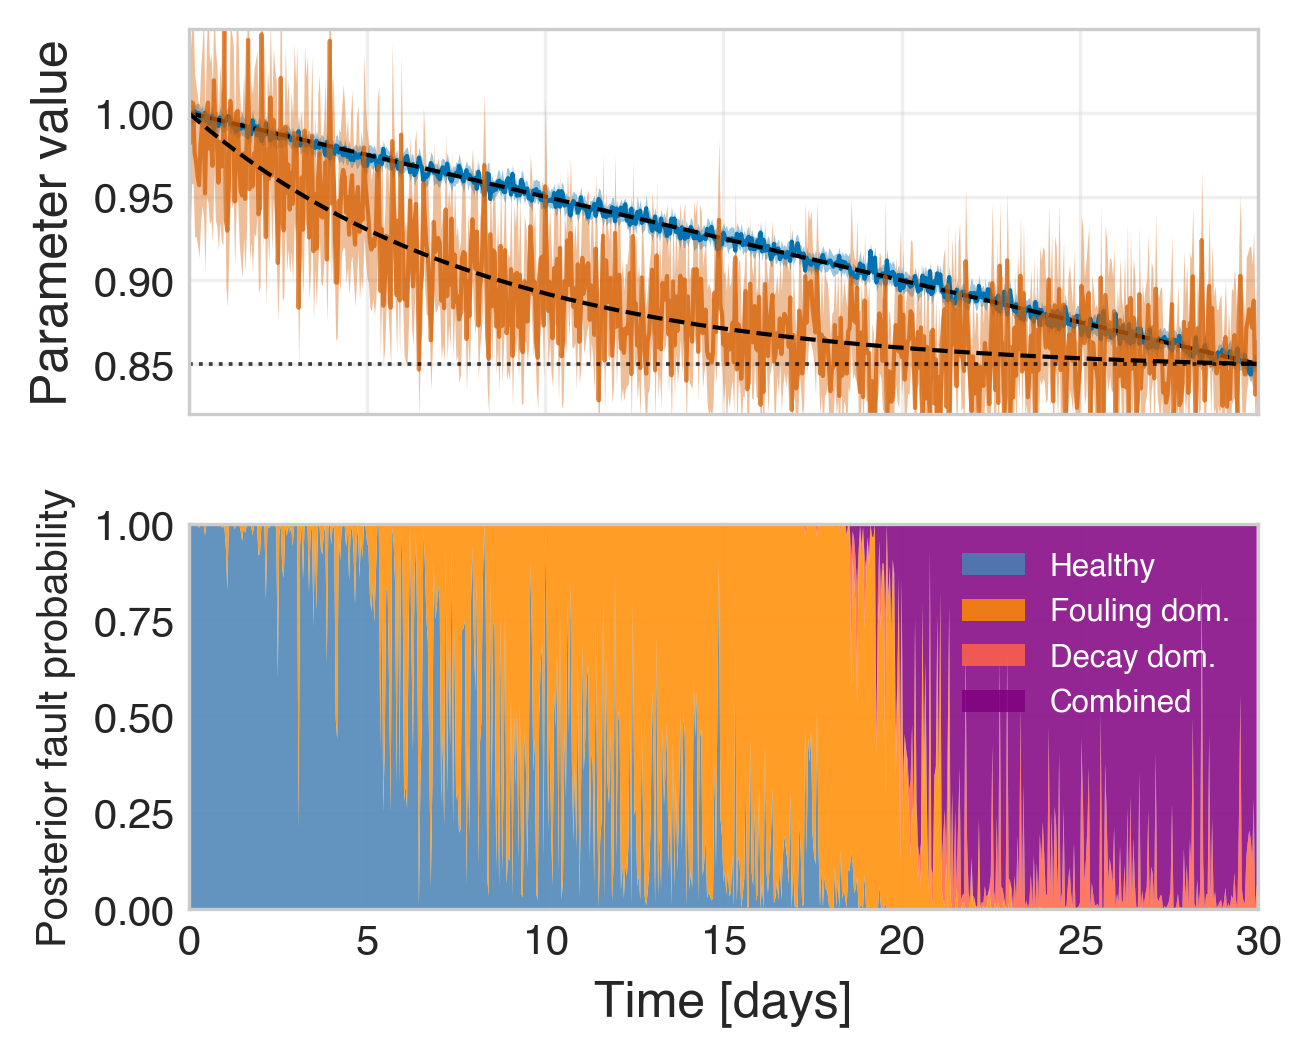
\includegraphics[width=0.99\linewidth]{10_degradation_tracking}
  \caption{30-day sequential degradation tracking for System~I (720 consecutive
    60-min windows, $\alpha$ decay and $\beta$ fouling, both
    reaching 0.85 at day 30).
    The upper panel overlays the amortised SBI posterior means and 90\% credible
    intervals for $\alpha(t)$ and $\beta(t)$ on their true degradation profiles,
    with the classification threshold shown as a dotted reference line.
    The lower panel shows the corresponding posterior fault-class probabilities
    for each window, revealing the healthy-to-fouling and fouling-to-combined
    transitions as the stream crosses the decision thresholds.}
  \label{fig:tracking}
\end{figure}
% ------------------------------------------------------------------
To demonstrate operational utility, the trained NSF posterior is applied
to a synthetic 30-day monitoring stream consisting of 720 consecutive 60-minute
observation windows.
The degradation profile follows a linear catalyst decay
$\alpha(t) = 1 - 0.15\,(t/720)$ and a
Kern--Seaton~\citep{KernSeaton} (asymptotic) fouling curve
$\beta(t) = 1 - b\,(1 - e^{-t/200})$, with $b$ chosen so that $\beta(720)=\alpha(720)$
exactly,
so that by the end of the
monitoring period $\alpha^* = \beta^* = 0.85$ --- a milder target than an earlier
version of this scenario, chosen to match the mild-fault severity used elsewhere in
this manuscript's scenario design (e.g.\ Sc\,4, Table~\ref{tab:scenario_results}).
Because the asymptotic $\beta(t)$ falls faster than the linear $\alpha(t)$ at early
times, $\beta$ crosses the classification threshold first (around day 8.7) and
$\alpha$ later (around day 20), so the stream passes through a genuine
\emph{healthy~$\to$~fouling-dominant~$\to$~combined} progression.
Each window is processed independently with no temporal prior propagation
performed, making the tracker stateless and directly deployable in an existing 
process historian without bespoke integration.

The SBI tracker achieves $\mathrm{MAE}_\alpha = 0.0027$ and
$\mathrm{MAE}_\beta = 0.0206$ over the full 30-day run, completing all 720
windows in 8.5~s (wall clock, CPU inference) --- an amortisation speedup of
approximately 38{,}900$\times$ relative to an equivalent per-window NUTS estimate.
For comparison, EKF and UKF achieve
$\mathrm{MAE}_\alpha = 0.0232/0.0249$ and $\mathrm{MAE}_\beta = 0.0652/0.0903$
respectively, roughly an order of magnitude higher $\alpha$ error and
$3$--$4\times$ higher $\beta$ error than SBI, consistent with the genuine
closed-loop information-deficit evidence discussed in
Section~\ref{sec:identifiability}.
Fault classification is correct in 84.4\% of windows overall; this aggregate masks a
non-monotonic pattern that is itself informative: accuracy is lowest ($\approx80\%$)
during the two phases where the stream crosses a genuine classification-threshold
boundary, and highest ($\approx94\%$) once both parameters are unambiguously on the
fault side of their thresholds.

% =============================================================
\section{Results: System~II --- Luyben Reactor-Column-Recycle Plant}
\label{sec:results_system2}
% =============================================================

%Results for System~II (Wu et al.~\citeyearpar{Wu2003}) are presented belowfollowing the same structure as Section~\ref{sec:results_system1}: summarystatistics, structural identifiability, fault classification, and degradation tracking.  
For System II, the central finding is that the 66-D summary representation 
introduces apparent joint parameter couplings that are not plant-level non-
identifiabilities under a raw-trajectory Fisher-information check. In contrast, 
reactor-temperature masking by Loop 1 remains a genuine representation-independent 
information loss.

\subsection{Physics-Informed Summary Statistics for System~II}
\label{sec:wu_summary_stats}
% ---------------------------------------------------------------------------

Similar to System I, each 2-hour observation window is compressed into
a 66-dimensional summary-statistic vector prior to passing it to the neural
density estimator. The complete feature definitions, per-parameter 
mutual-information rankings, and PCA-based separability analyses are detailed
in the Supporting Information.

Among these features, two physics-informed proxies carry much of the identifying information. The System II analogue of $s_{U\!A}$ for System I (Eq.~\eqref{eq:ua_proxy}), is given by:

\begin{equation}
  s_{UA,r} = \frac{T_r - T_j}{Q_j} \propto (\beta_r\!\cdot\!U\!A_r)^{-1} \, .
  \label{eq:wu_ua_proxy}
\end{equation}
%
Under Loop~1 PI control,
$T_r \approx T_\mathrm{sp}$ and the numerator encodes the jacket temperature
drop driven by fouling, while the denominator normalises by the controller
output.  The normalised recycle flow deviation
%
\begin{equation}
  s_{F_R} = F_{R,\mathrm{norm}} - 1
  \label{eq:wu_fr_proxy}
\end{equation}
%
provides the primary snowball indicator. Any reduction in per-pass conversion (lower $\alpha$ or $\eta_\mathrm{col}$) drives $F_{R,\mathrm{norm}}$ above 1.
Because both parameters raise $s_{F_R}$ in the same direction, $s_{F_R}$ alone cannot distinguish catalyst decay from column-efficiency loss and a confound is to be expected. The identifiability analysis in Section~\ref{sec:wu_identifiability} investigates this directly.

\subsection{Fault Classification}
\label{sec:wu_fault_class}
% ---------------------------------------------------------------------------

The production NSF posterior was applied to the 14 closed-loop System II fault
scenarios using the unit-level posterior-mass rule defined in Section IV A.
Classification is reported at the fault-unit level because operational
decisions concern whether the reactor, column, feed system, or multiple
units are degraded, rather than only which individual parameter crossed the 
threshold.

% ------------------------------------------------------------------
\begin{table*}[tbp]
\centering
\caption{Unit-level fault classification results for System~II
  (14 scenarios, 30 replicates for the production NSF posterior,
  $\theta_\mathrm{thr}=0.85$). Per-class F\textsubscript{1} is the
  harmonic mean of precision and recall across all replicates in each fault-unit category.}
\label{tab:wu_classification}
\small
\begin{tabular}{llrl}
\toprule
Fault unit & Scenarios & $F_1$ & Note \\
\midrule
Healthy  & W1                  & 0.667 & Some healthy replicates border the threshold \\
Reactor  & W2--W6, W11, W15    & 0.948 & Near-perfect despite $(\alpha,\beta_r)$ corr = 0.998 \\
Column   & W7, W9              & 1.000 & $\eta_\mathrm{col}$ and $\xi_\mathrm{reb}$ well-identified \\
Feed     & W10                 & 0.000 & Artefact~3 confound with $\alpha$ (Section~\ref{sec:wu_artifact3}) \\
Multi    & W12, W13, W16       & 0.854 & W13 weak (7/30): feed+reactor compound, Artefact~3 \\
\midrule
\multicolumn{2}{l}{Overall macro-F1} & 0.694 & 87.4\% accuracy \\
\bottomrule
\end{tabular}
\end{table*}
% ------------------------------------------------------------------

% ------------------------------------------------------------------
\begin{figure}[tb]
  \centering
  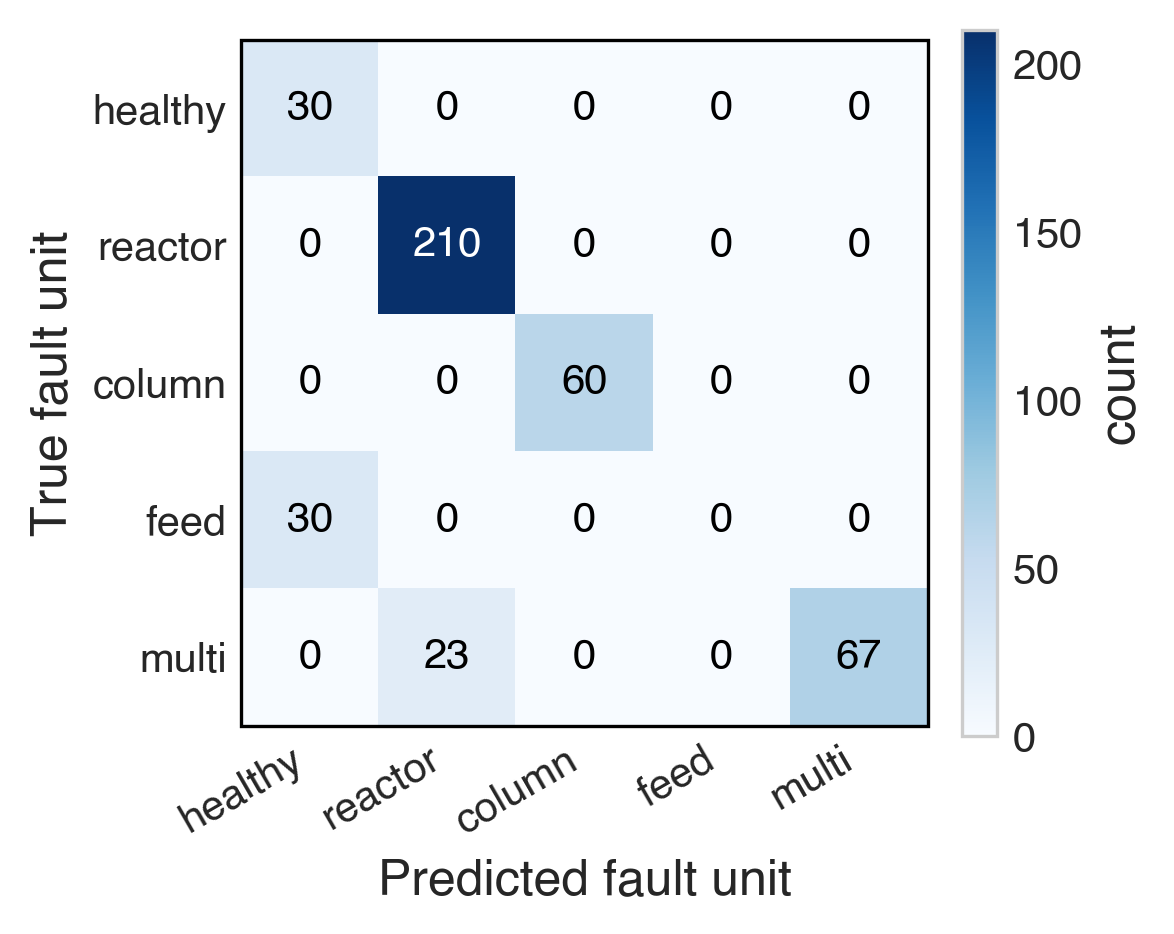
\includegraphics[width=0.9\linewidth]{nb31_confusion_matrix}
  \caption{Unit-level fault confusion matrix for System~II (14 scenarios,
    30 replicates each). Rows: true fault unit; columns: predicted fault unit.
    Reactor and column faults are reliably detected. Feed-fault scenarios
    (W10, W13) are predominantly misclassified as reactor or compound faults as a 
    consequence of the representation-level $(\alpha, z_{A0,\mathrm{eff}})$
    confound identified in Section~\ref{sec:wu_artifact3}.}
  \label{fig:wu_confusion}
\end{figure}
% ------------------------------------------------------------------

Overall unit-level classification accuracy is 87.4$\%$, with macro-F1 = 0.694. 
Performance is uneven across units: reactor and column faults are detected
reliably, whereas feed faults fail under the present representation.
Per-unit results are summarised in Table~\ref{tab:wu_classification} and the
confusion matrix is shown in Figure~\ref{fig:wu_confusion}.


Breaking down the performance by functional unit reveals how representation 
artefacts impact downstream diagnosis. 
Reactor and column faults are detected reliably. Reactor scenarios are correctly classified despite parameter-level ambiguity between $\alpha$ and $\beta_r$, because both parameters map to the same reactor unit. Column scenarios are also classified reliably, including the cross-unit W12 case. In contrast, the feed-purity scenario W10 is misclassified in all 30 replicates, indicating that the present representation does not support reliable feed-fault attribution.

%\paragraph{\textbf{Comparison against the Extended Kalman Filter (EKF).}}
Table~\ref{tab:wu_ekf_classification} places the SBI classification alongside 
the baseline EKF estimates. The EKF structurally cannot observe $z_{A0,\mathrm{eff}}$ 
(estimating only $[\alpha,\beta_r,\eta_\mathrm{col}]$), offering no comparison point at W10. 
Where the EKF does produce estimates, two distinct regimes emerge. At the 
near-snowball scenarios W12 and W15 ($\alpha = 0.75$ and $\alpha = 0.58$ respectively), 
the EKF achieves only 3\% empirical coverage on $\alpha$,consistent with a failure of local Gaussian linearisation under strong non-linear recycle dynamics near the tipping point. SBI, conversely, achieves 100\% coverage at W15. 
At W11, the EKF's 0\% coverage is a tuning-sensitive pitfall rather than evidence 
of a genuine degeneracy, as an independently re-tuned EKF with raw-trajectory 
access recovers both parameters to $<2$\% error (Section~\ref{sec:wu_artifact2}). 
Crucially, SBI's unit-level classification remains correct across all three of these 
scenarios (W11, W12, W15) regardless of baseline tuning sensitivities.

% ------------------------------------------------------------------
\begin{table*}[tbp]
\centering
\caption{SBI vs.\ EKF at the scenarios used to illustrate fault-classification
  robustness (System~II). The augmented EKF
  (Section~\ref{sec:wu_sequential}) estimates only $[\alpha,\beta_r,\eta_\mathrm{col}]$ whereas
  $\xi_\mathrm{reb}$ and $z_{A0,\mathrm{eff}}$ are outside its augmented state and are therefore unobservable to it by construction, not merely difficult to estimate.}
\label{tab:wu_ekf_classification}
\small
\begin{tabular}{llllll}
\toprule
Scenario & True fault unit & SBI classification           & EKF estimate & EKF 90\% coverage & Note \\
\midrule
W10 & Feed ($z_{A0,\mathrm{eff}}=0.75$)  & Misclassified,  & --- & --- & $z_{A0,\mathrm{eff}}$ not in EKF's  \\
    &                                    & $F_1=0.000$ &  & & augmented state \\

W11 & Reactor ($\alpha=\beta_r=0.80$)    & Correct, 30/30 & $\hat\alpha=0.907$,& 0\% & Tuning-sensitive; see Artefact~2 \\
       &                                     & & $\hat\beta_r=0.986$ &  & \\
W12 & Multi ($\alpha=0.75$)              & Correct, 30/30 & $\hat\alpha\approx1.19$ & 3\% & Snowball nonlinearity \\
W15 & Reactor ($\alpha=0.58$)            & Correct, 30/30 & $\hat\alpha=0.990$ & 3\% & Near snowball tipping point \\
\bottomrule
\end{tabular}
\end{table*}
% ------------------------------------------------------------------



% ---------------------------------------------------------------------------
\subsection{Structural Identifiability Analysis}
\label{sec:wu_identifiability}
% ---------------------------------------------------------------------------


% ------------------------------------------------------------------
\begin{figure}[tb]
  \centering
  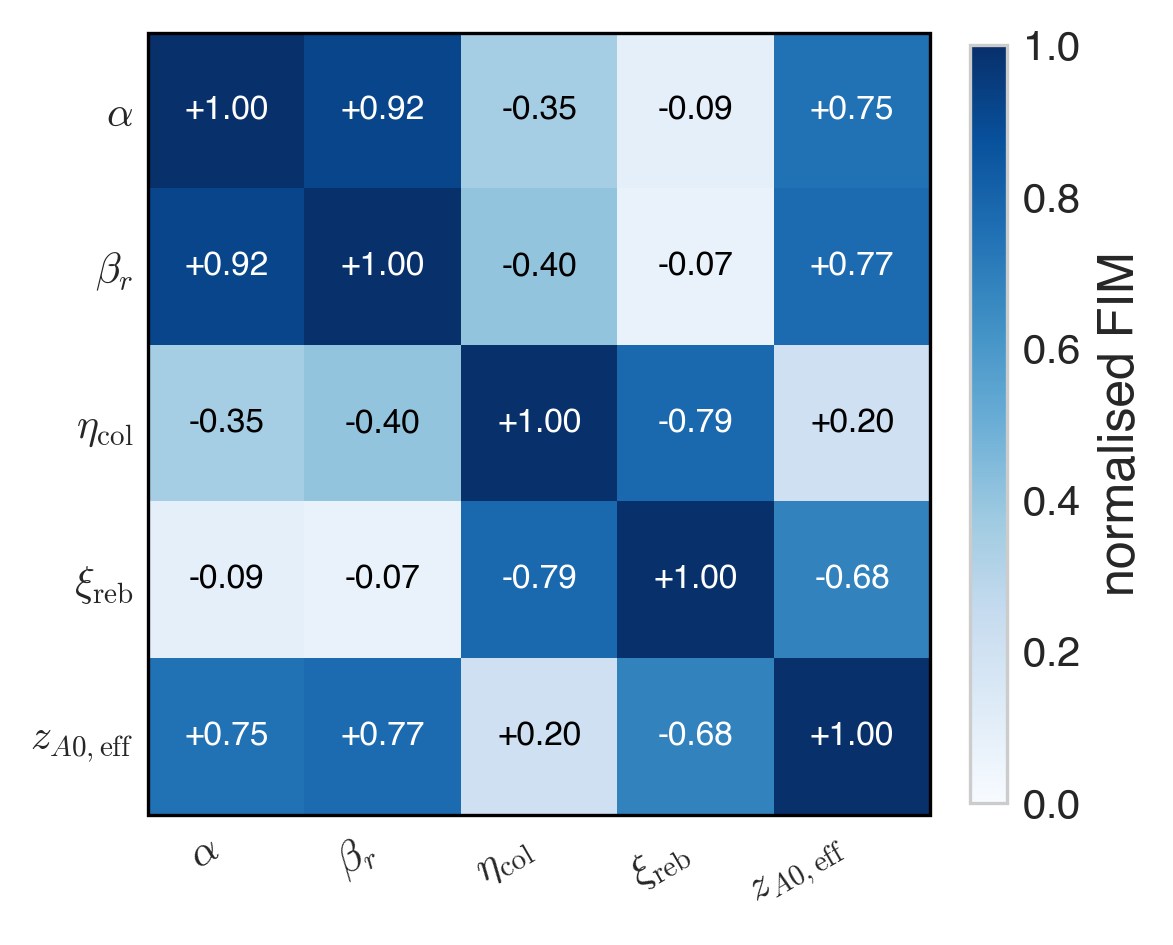
\includegraphics[width=0.97\linewidth]{nb23_fim_heatmap_single}
  \caption{Normalised $5\times5$ Fisher information 
  matrix at System II nominal
    operating point.
    Entries show the signed, normalised parameter coupling at the nominal operating point, with colour intensity indicating absolute information coupling strength. The strong positive $\alpha-\beta_r$
  off-diagonal term highlights a dominant identifiability confounding between reactor degradation and reactor heat-transfer loss, while the remaining structure shows weaker or more localized couplings among column efficiency, reboiler efficiency, and feed composition.
  The high off-diagonal $+0.93$ for $(\alpha,\beta_r)$
    under the full feature set is investigated as a potential joint degeneracy in
    Sections~\ref{sec:wu_artifact1}--\ref{sec:wu_artifact3}.}
  \label{fig:wu_fim}
\end{figure}
% ------------------------------------------------------------------

System II raises a different identifiability question from System I. Loop 1 masks reactor-temperature sensitivity in the same way as the CSTR controller, but the dominant difficulty in System II is not only scalar information loss. The 66-D summary representation also introduces apparent joint couplings between degradation parameters.\\
To distinguish plant-level non-identifiability from representation-induced coupling, we recompute the local FIM for each candidate confound using raw, unaggregated trajectories of the already observed channels at the same operating point. We compare normalized off-diagonal entries, Cramér-Rao standard deviations, and FIM condition numbers across the summary and raw representations. A substantial reduction in normalized coupling accompanied by improved conditioning indicates that the compressed representation has discarded locally distinguishing information. The test is local and information-theoretic: it identifies available information in the measured signals, but does not guarantee recovery by a finite-capacity amortised estimator.
The RT-FIM check is computationally inexpensive relative to posterior training. At the replicate count used here, one representation at one operating point requires $\mathcal{O}(10^2)$ simulator calls, compared with $\mathcal{O}(10^4)$ simulations for the amortised posterior training.\\

\subsubsection{Artefact 1: Restricted-channel coupling between
  \texorpdfstring{$\alpha$}{alpha} and
  \texorpdfstring{$\eta_\mathrm{col}$}{eta_col}}
\label{sec:wu_artifact1}

The apparent $\alpha-\eta_{col}$ confound appears only when the analysis is restricted to 
recycle-flow-derived features. Both parameters affect $F_{R,\mathrm{norm}}$ through
conversion and recycle coupling, so this restricted representation produces an
elongated ridge. Once the already measured reboiler channels, $T_\mathrm{reb}$ and
$Q_\mathrm{reb}$, are included in the full feature set, the ambiguity is removed: 
posterior correlations remain below 0.15 and the $\eta_{col}$ 90$\%$ credible 
interval width is approximately 0.01-0.02 across the tested scenarios. This is 
therefore a restricted-channel artefact, not a plant-level non-identifiability.
Consistent with this interpretation, scenario W12 is classified correctly as a compound reactor-column fault in all 30 replicates.

\subsubsection{Artefact 2: Temporal-aggregation confound between
  \texorpdfstring{$\alpha$}{alpha} and
  \texorpdfstring{$\beta_r$}{beta_r}}
\label{sec:wu_artifact2}

The strongest summary-level confound is the reactor-side pair $\alpha-\beta_r$. At W11, the 66-D summary representation gives a posterior correlation of +0.998 and a FIM-normalized off-diagonal of approximately +0.85 to +0.90, indicating an almost one-dimensional ridge.
The raw-trajectory FIM indicates that this coupling is not intrinsic to the measured plant signals. Recomputing the FIM on the unaggregated trajectories of the already observed reactor-side channels collapses the normalized off-diagonal to approximately zero. The condition number falls from 3.45 $\times$ 10$^3$ under the 66-D summaries to 5.34 under the raw trajectory, showing that the improvement is not merely a rotation of the uncertainty ellipse but a genuine local gain in parameter distinguishability.
Feature decomposition indicates that whole-window statistics of the cooling duty $Q_j$ dominate the summary-level coupling. This is physically plausible: both lower catalyst activity and lower jacket conductance are compensated by Loop 1 through changes in $Q_j$. Whole-window means and quantiles preserve the common level shift but discard transient shape information that distinguishes the two mechanisms.
This confound is therefore a temporal-aggregation artefact. However, it is not automatically solved by any raw-data estimator: the retuned EKF with raw-model access resolves the pair, whereas the tested CNN-SBI posterior does not. The RT-FIM result should therefore be interpreted as local information-theoretic recoverability, not as a guarantee of amortised SBI recovery.\\

\subsubsection{Artefact 3: Composition-confound between reactor faults and feed
  purity}
\label{sec:wu_artifact3}

The feed-purity parameter $z_{A0,\mathrm{eff}}$ shows strong summary-level coupling with reactor-side degradation at degraded operating points. 
For example, at the W2 operating point the $\alpha$-$z_{A0,\mathrm{eff}}$ 
FIM off-diagonal is approximately -0.89 under the 66-D representation, 
compared with approximately -0.12 at nominal conditions.
The raw-trajectory FIM removes this local coupling: the corresponding off-diagonal 
falls to approximately -0.07, and the condition number decreases from 4.36 $\times$ 
10$^3$ to 5.48. The analogous $\beta_r$-$z_{A0,\mathrm{eff}}$ coupling at the W5 
operating point shows the same pattern, with the condition number decreasing from 
41.4 to 5.24. Thus, the feed-reactor coupling is also representation-induced rather 
than a plant-level non-identifiability.\\
Unlike Artefact 2, this representation artefact is operationally severe. The 
confused parameters belong to different fault units, so the representation-level 
ambiguity corrupts unit-level classification rather than only parameter attribution 
within the same unit. This explains why W10 feed faults are misclassified in all 30 
replicates and the feed class has F1 = 0.000.

\textit{Raw-trajectory CNN posterior as a practical recovery test.}
A CNN-embedding SBI posterior was trained on raw 120 $\times$ 9 trajectories to test 
whether an amortised neural estimator could exploit the information identified 
by RT-FIM. The results are mixed. Artefact 1 remains resolved, and the 
$\alpha$-$z_{A0,\mathrm{eff}}$ correlation associated with Artefact 3 collapses 
from approximately +0.99 to near zero. However, Artefact 2 remains unresolved: 
the $\alpha$-$\beta_r$ posterior correlation remains above +0.99 across tested
seeds and operating points.\\
The CNN posterior also fails to improve feed-fault classification. Feed F1 remains 
0.000, although the failure mechanism changes: under the hand-crafted posterior,
feed faults are masked by the $\alpha$-$z_{A0,\mathrm{eff}}$ correlation, while 
under the CNN posterior they are dominated by a systematic downward bias in 
$\alpha$. 
Consequently, the CNN result reinforces the distinction between local 
information availability and practical amortised recovery. RT-FIM can show that the 
raw signals contain distinguishing information, but estimator architecture, training 
budget, and bias determine whether that information is actually used.
This failure does not invalidate the plant-wide SBI framework; rather, it identifies feed attribution as the unit for which the current measurements, representation, or decision rule are insufficient.\\
Together, the three cases show that summary-induced confounds should not be
interpreted solely by their Fisher-information magnitude. Artefacts 2 and 3 have
comparable summary-level coupling, but their classification consequences are 
opposite. The $\alpha$-$\beta_r$ ambiguity is mostly benign for unit-level diagnosis because
both parameters belong to the reactor unit. The $\alpha$-$z_{A0,\mathrm{eff}}$
ambiguity is severe because it crosses the reactor-feed unit boundary. Thus, the 
operational severity of a representation artefact depends on the fault taxonomy
used for decision-making, not only on local parameter coupling.

\subsection{30-Day Sequential Degradation Tracking}
\label{sec:wu_sequential}
\begin{figure}[t]
    \centering
    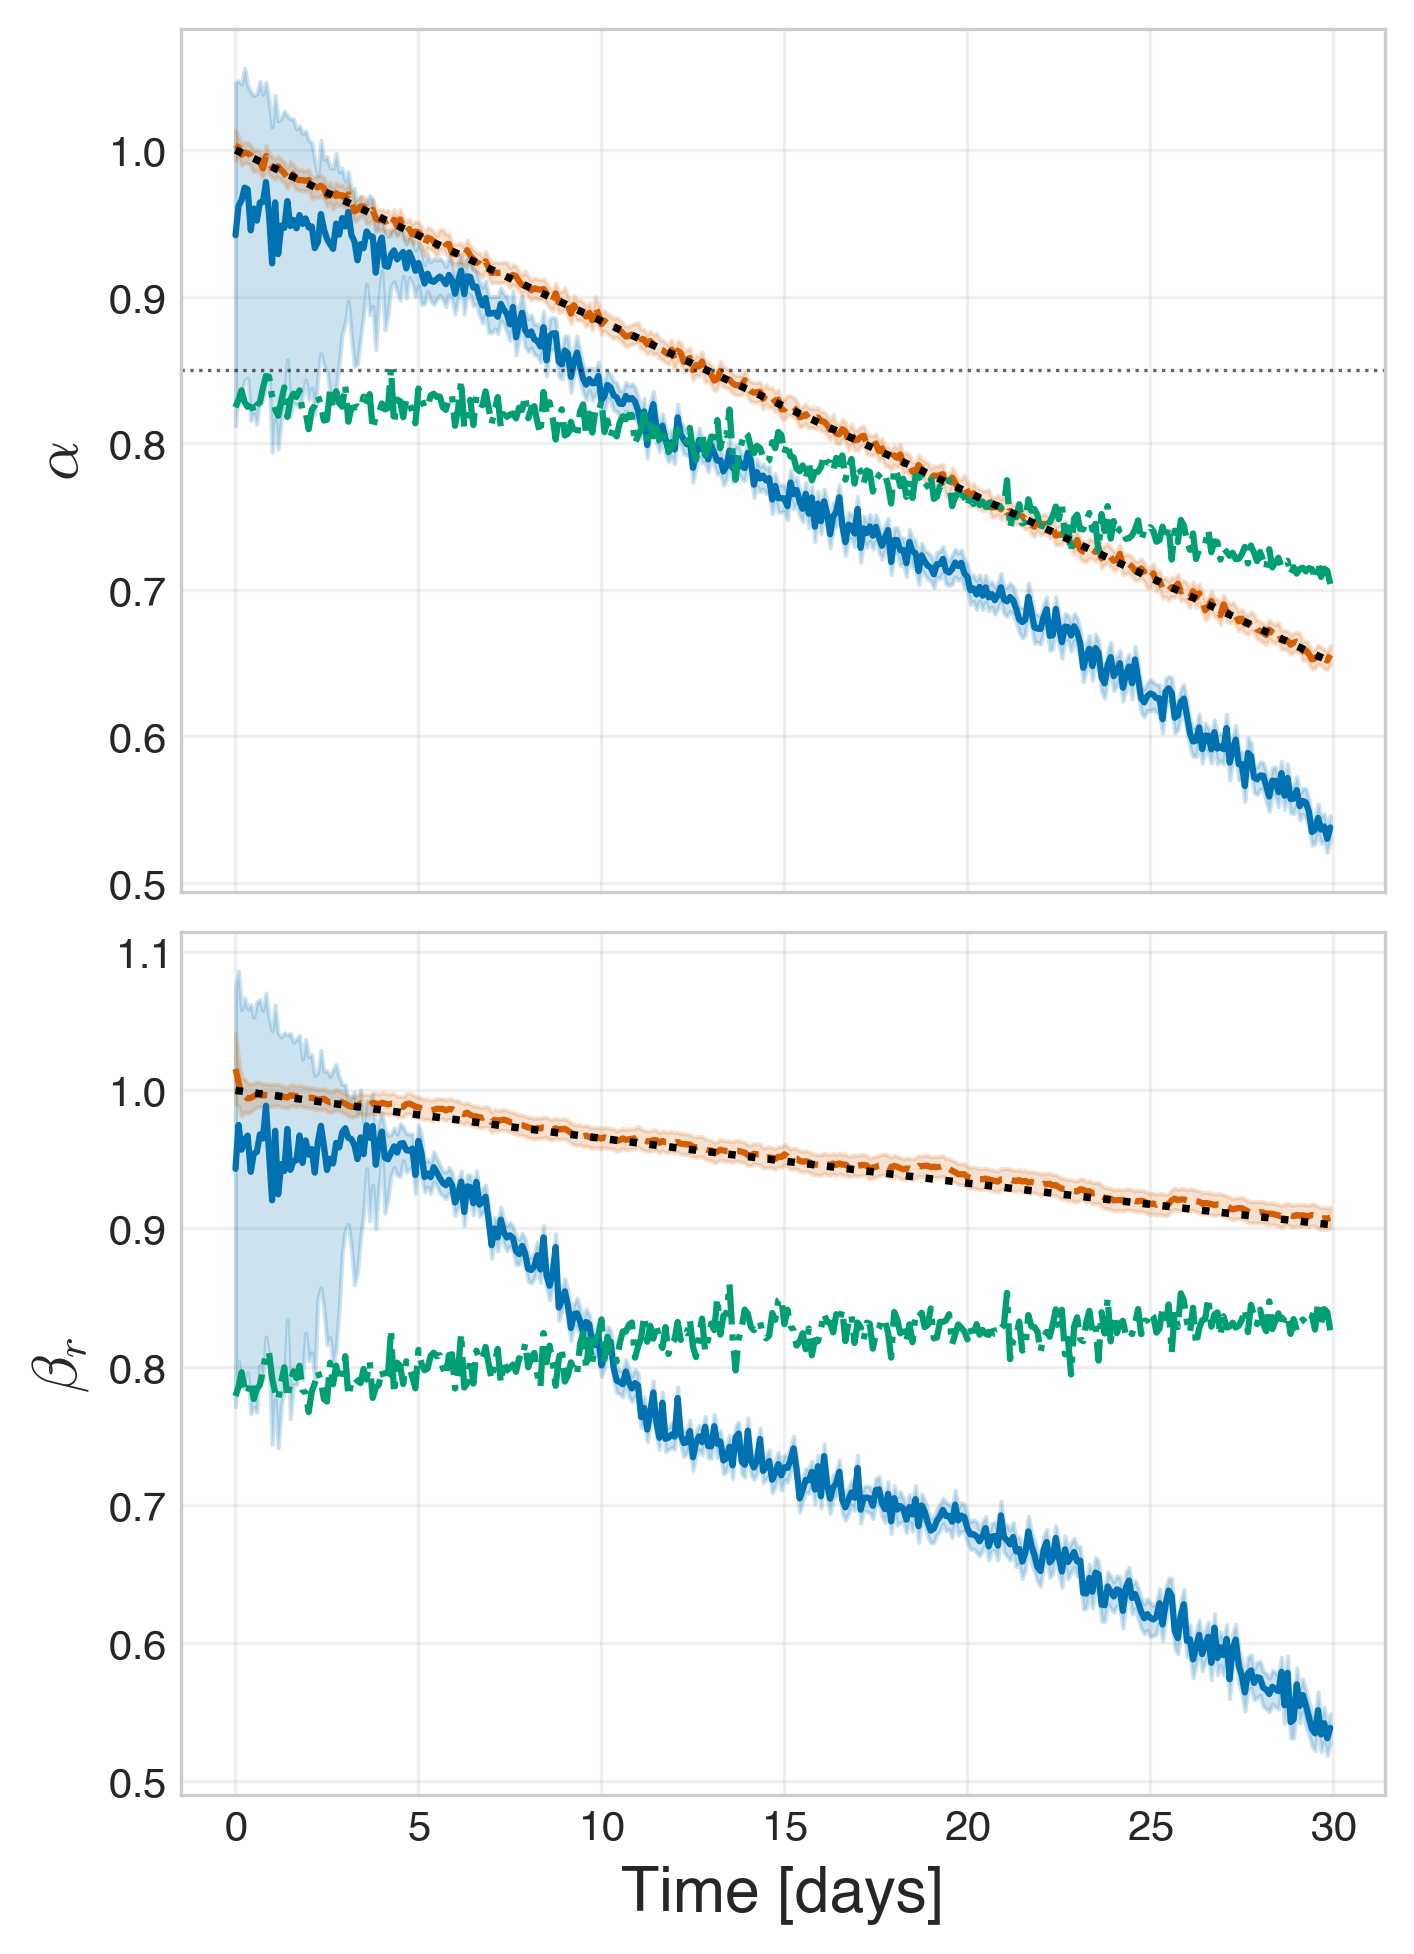
\includegraphics[width=0.95\linewidth]{nb27_sequential_tracking.png}
    \caption{Sequential System II degradation tracking over 30 days. The true trajectories for catalyst activity 
    $\alpha$ and $\beta_r$ and reactor heat-transfer factor 
  are compared with independent amortised SBI estimates (blue), recursive EKF estimates (orange), and CNN-embedding SBI posterior means (green) across 360 two-hour windows. Shaded bands show 90$\%$ intervals for SBI and EKF only. The EKF tracks both slowly varying parameters closely, while the amortised SBI methods show larger bias and delayed response, especially for $\beta_r$, illustrating the difficulty of recovering gradual degradation from independent window-level posterior inference.}
    \label{fig:sysII_track}
\end{figure}

The calibrated  posterior is applied to a synthetic 30-day
monitoring stream of 360 consecutive 2-hour observation windows, each
processed independently (no temporal state carried between windows). The
degradation profile follows a linear catalyst decay reaching $\alpha \approx
0.65$ and a Kern--Seaton fouling curve reaching $\beta_r \approx 0.90$ by day
30, with $\eta_\mathrm{col}$, $\xi_\mathrm{reb}$, and $z_{A0,\mathrm{eff}}$
held at their healthy values throughout. Results are shown in 
Figure~\ref{fig:sysII_track}.

In this sequential tracking experiment, the EKF outperforms the amortised SBI
posterior. This result should be interpreted as a limitation of the present
per-window summary representation rather than as a general limitation of SBI. 
Control experiments (Supporting
Information~\S{}S11) rule out any advantage from accumulating information
across the 360-window run, and instead trace the gap to the EKF's privileged
access to the raw, unaggregated trajectory through the exact ODE model
consistent with Artefact~2 (Section~\ref{sec:wu_artifact2}). The CNN-embedding
posterior (Supporting Information Section~S10) narrows part of this gap
($\mathrm{MAE}_{\beta_r}$ improves to $0.139$) but not all of it
($\mathrm{MAE}_\alpha$ worsens to $0.067$), both still an order of magnitude
short of the EKF. SBI remains substantially faster per window (15~ms vs.\
25.9~ms for the EKF). %Full control experiments, the tracking figure, and per-window metrics are given in Supporting Information~\S{}S11.
% Full CNN results --- SBC calibration, per-scenario correlations, and 30-day
%tracking --- are given in Supporting Information Section~S10.


% ===========================================================================
\section{Discussion}
\label{sec:discussion}
% ===========================================================================

\subsection{One Genuine Limit, Three Representation Artefacts}
\label{sec:disc_limit_artefacts}

The two systems separate two qualitatively different sources of diagnostic 
difficulty. The first is genuine closed-loop information loss: integral control 
removes the primary controlled-variable signature of thermal degradation. This 
effect appears strongly for $\beta$ in System I and more mildly for $\alpha$
and $\beta_r$ in System II. Because it is present in the raw trajectories and
reproduced across inference methods, it cannot be removed by changing summary 
statistics.\\
The second source is representational. In System II, the 66-D summary representation 
creates apparent joint couplings that weaken or disappear under the RT-FIM check. 
These couplings are therefore not plant-level non-identifiabilities, although they 
may still harm practical SBI inference and fault classification. The distinction is 
operationally important: representation artefacts call for improved features, 
learned embeddings, or revised decision rules, whereas genuine closed-loop masking 
requires new measurements or deliberate excitation.\\
These results show that plant-wide SBI posteriors must be evaluated against the fault
 taxonomy used for operational decisions, not only against parameter-level identifiability metrics.

\subsection{Why Amortised SBI Is the Appropriate Instrument for This Problem Class}
\label{sec:disc_why_sbi}
SBI is useful for closed-loop plant-wide fault identification because the simulator
 is available but an explicit likelihood over multi-unit, feedback-controlled observation windows is not. Its main advantage
over Gaussian filters is not universal accuracy, but the ability to
represent joint, non-Gaussian posterior structure and to amortise
inference across repeated monitoring windows. This is particularly
valuable when the posterior geometry itself is diagnostically meaningful,
as in the distinction between unit-benign and unit-severe confounds.
However, the results also show that SBI is not uniformly superior to
model-based estimators. In System II tracking, a tuned EKF with raw-model
access outperforms the amortised summary-statistic posterior. Thus, the
practical value of SBI is strongest when likelihood construction is difficult,
posterior geometry is non-Gaussian, or per-window optimisation is
undesirable, not when an exact model and well-tuned recursive estimator are 
available.


\subsection{EKF Failure and Success Regimes}
\label{sec:disc_ekf_regimes}

The EKF comparisons indicate that no universal ranking between SBI and classical 
estimators is appropriate. EKF failures near W12/W15 reflect the limits of local 
Gaussian linearisation under strong recycle nonlinearity, while the W11 failure is 
tuning-sensitive rather than structural. Conversely, in 30-day System II tracking, a 
well-tuned EKF with exact raw-model access outperforms the current per-window SBI 
posterior. Recursive pooling of biased per-window SBI posteriors does not solve this 
problem because it compounds systematic representation bias rather than averaging 
independent noise. The relevant distinction is therefore not SBI versus EKF in 
general, but amortised summary-based inference versus raw-trajectory model-based 
estimation under each operating regime.

% ===========================================================================
\section{Summary and Conclusions}
\label{sec:conclusions}
% ===========================================================================


This work demonstrates amortised SBI as a framework for Bayesian fault identification
in closed-loop chemical processes, including a plant-wide reactor-column-recycle system
with multiple interacting units and decentralized PI control.\\
In the PI-controlled CSTR, jacket fouling is intrinsically harder to estimate than catalyst
activity because integral temperature control removes the primary temperature signature
of heat-transfer degradation. Under the original training protocol, a $\beta$ bias
appeared in all of SBI, CNN-SBI, MCMC, EKF, and UKF; however, SBI, CNN-SBI, and MCMC
shared a training/evaluation initial-condition mismatch (a protocol-induced inference
artefact, not a plant property), and correcting it removes nearly all of their bias
while EKF and UKF's bias --- unaffected by the mismatch, since their filter state initialises
from the observed data directly --- remains. The persistent EKF/UKF bias is therefore
the more credible remaining evidence of a genuine, though smaller than originally reported, 
closed-loop information deficit for $\beta$.

In the reactor-column-recycle benchmark, the 66-D summary representation produces three
apparent joint confounds. Raw-trajectory FIM analysis shows that these are locally 
recoverable from the already observed signals and are therefore representation artefacts 
rather than plant-level non-identifiabilities. However, their downstream consequences differ:
reactor-side ambiguity is benign for unit-level classification, whereas feed-reactor ambiguity
collapses feed-fault detection.

The results show that SBI is useful not because it universally outperforms classical
estimators, but because it provides joint posterior structure and amortised inference
in settings where likelihood construction is difficult. Conversely, when an exact model
and raw trajectory are available, a well-tuned EKF can outperform the current SBI
implementation. Practically, representation artefacts call for richer features, learned
embeddings, or additional decision rules, while genuine closed-loop masking requires new
measurements or deliberate excitation. The present System II implementation therefore
demonstrates plant-wide SBI fault identification for reactor and column faults, while
identifying feed-fault attribution as the remaining limitation requiring richer
measurements, less lossy representations, or revised decision rules.


\section{Data and code availability}
The code and experiments used in this paper are available on GitHub
at: \nolinkurl{https://github.com/XXXXX}.\\

\section{CRediT authorship contribution statement}
%\section{authorship contribution statement}
\textbf{Simone Casolo}: Writing, methodology, formal analysis, conceptualization.
\textbf{Alexander J. Stasik}: Review $\&$ editing, supervision, methodology.
\textbf{Signe Riemer-S\o rensen}: Review $\&$ editing, supervision, methodology, conceptualization.\\

\section{Declaration of competing interest}
The authors declare that they have no known competing financial interests or personal relationships that could have appeared to influence the work reported in this paper.

\section{Acknowledgements}
This publication has been funded by the SFI NorwAI, (Centre for Research-based Innovation, 309834). The authors gratefully acknowledge the financial support from the Research Council of Norway and the partners of the SFI NorwAI.

\bibliographystyle{apsrev4-2}
%\bibliographystyle{elsarticle-harv} 
\bibliography{references}

\end{document}
